% March 2015
% Autor: Mandy Vogel
% introduction

\documentclass[xcolor={table},c]{beamer}
%\usetheme[backgroundimagefile=mathe]{diepen}
\usetheme{Singapore}
% \useoutertheme{miniframes}

%\setbeamerfont{block title}{size=\small,series=\bfseries}
%\setbeamerfont{block body}{size=\footnotesize}

% \usecolortheme{beetle}
\usepackage{linkimage}

%\usepackage{handoutWithNotes}
%\pgfpagesuselayout{3 on 1 with notes}[a4paper,border shrink=5mm]

\begin{document}

\title{Hadley's Packages}   
\author{Mandy Vogel} 
\date{\today}

\AtBeginSection{
  \begin{frame}<beamer>[allowframebreaks,t]{Table of Contents}
    \tableofcontents[currentsection]
  \end{frame}}

\begin{frame}
\titlepage
\end{frame}

\begin{frame}[allowframebreaks,t]{Table of Contents}
\frametitle{Table of Contents}\tableofcontents
\end{frame}



\section{ggplot2 - Part 1}
\subsection{The ggplot2 graphics model}

\begin{frame}[fragile]\frametitle{Structure of a ggplot Object}
begin with an empty object to see the structure:
\begin{verbatim}
> po <- ggplot()
> summary(po)
data: [x]
faceting: facet_null() 
\end{verbatim}
\end{frame} 

\begin{frame}[fragile]\frametitle{Structure of a ggplot Object}
\scriptsize
\begin{verbatim}
> str(po)
  List of 9
  $ data       : list()
  ..- attr(*, "class")= chr "waiver"
  $ layers     : list()
  $ scales     :Reference class 'Scales' [package "ggplot2"] with 1 fields
  ..$ scales: NULL
  ..and 21 methods, of which 9 are possibly relevant:
  ..  add, clone, find, get_scales, has_scale, initialize, input, n,
  ..  non_position_scales
  $ mapping    : list()
  $ theme      : list()
  $ coordinates:List of 1
  ..$ limits:List of 2
  .. ..$ x: NULL
  .. ..$ y: NULL
  ..- attr(*, "class")= chr [1:2] "cartesian" "coord"
  $ facet      :List of 1
  ..$ shrink: logi TRUE
  ..- attr(*, "class")= chr [1:2] "null" "facet"
  $ plot_env   :<environment: R_GlobalEnv> 
  $ labels     : list()
  - attr(*, "class")= chr [1:2] "gg" "ggplot"
\end{verbatim}
\end{frame}


\begin{frame}[fragile]\frametitle{Structure of a ggplot Object}
Now we fill this structure - first the three main steps:
  \begin{itemize}
    \item the first argument to ggplot is \texttt{data}
    \item then specify what graphics shapes you are going to use to view the data (e.g. \texttt{geom\_line()} or \texttt{geom\_point()}).
    \item specify what features (or \texttt{aesthetics}) will be used (e.g. what variables will determine \texttt{x}- and \texttt{y}-locations) with the \texttt{aes()} function
    \item if these aesthetics are intented to be used in all layers it is more convenient to specify them in the \texttt{ggplot} object
  \end{itemize}
\end{frame}

\begin{frame}[fragile]\frametitle{Feed the Object}
  \begin{itemize}
  \item first we create a little sample data frame\small
\begin{verbatim}
> x1 <- 1:10; y1 <- 1:10; z1 <- 10:1
> l1 <- LETTERS[1:10]
> a <- 10; b <- (0:-9)/10:1
> ex <- data.frame(x=x1,y=y1,z=z1,l=l1,a=a,b=b)
> ex
    x  y  z l  a          b
1   1  1 10 A 10  0.0000000
2   2  2  9 B 10 -0.1111111
3   3  3  8 C 10 -0.2500000
4   4  4  7 D 10 -0.4285714
5   5  5  6 E 10 -0.6666667
6   6  6  5 F 10 -1.0000000
7   7  7  4 G 10 -1.5000000
8   8  8  3 H 10 -2.3333333
9   9  9  2 I 10 -4.0000000
10 10 10  1 J 10 -9.0000000
\end{verbatim}
  \end{itemize}
\end{frame}

\begin{frame}[fragile]\frametitle{Feed the Object}
  \begin{itemize}
  \item then create a \texttt{ggplot} object containing the data and some standard aesthetics (here we define the x and the y positions)
   \item add one or more geoms, we begin with  \texttt{geom\_point}
  \end{itemize}
\begin{verbatim}
> po <- ggplot(ex,aes(x=x1,y=y1))
> summary(po)
data: x1, y1, z1, l, a, b [10x6]
mapping:  x = x1, y = y1
faceting: facet_null() 
> p1 <- po + geom_point()
\end{verbatim}
\begin{center}
\linkimage{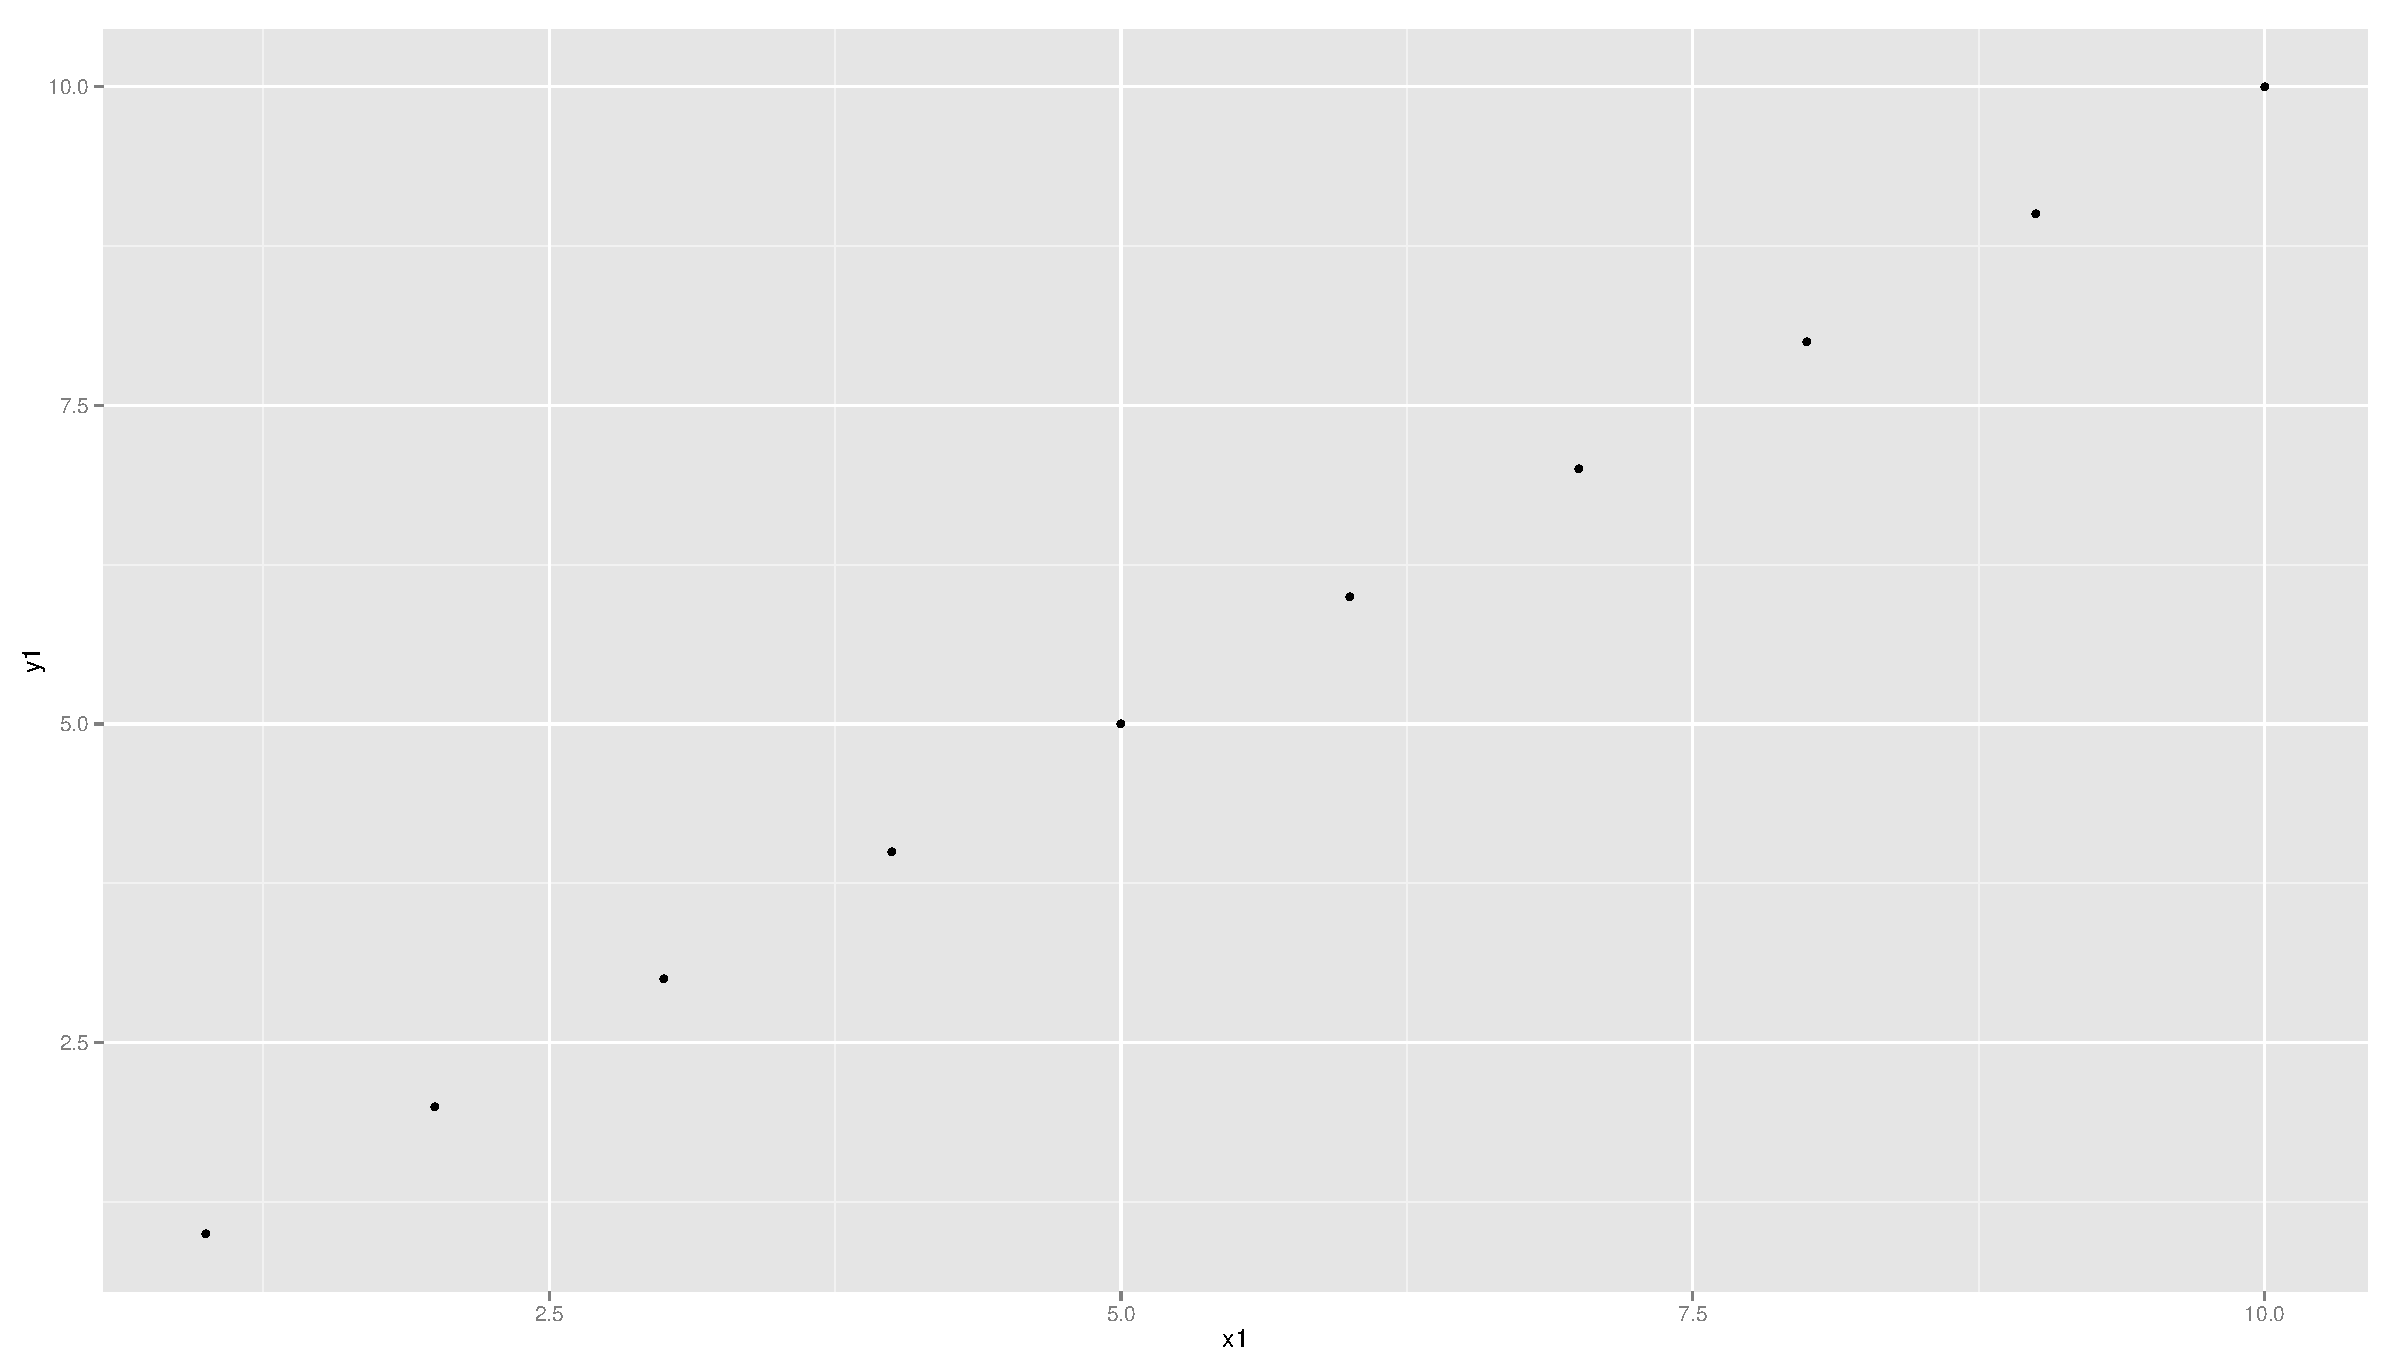
\includegraphics[width=6cm,height=4cm]{ggp1.pdf}}{ggp1.pdf}
\end{center}
\end{frame}

\subsection{\texttt{geometric objects} (Layers)}

\begin{frame}\frametitle{Layers}
  \begin{itemize}
    \item \texttt{ggplot()} creates an object - every "+" adds something to this object (change the object)
    \item the default method of ggplot() is \texttt{print()}, which creates the plot
    \item it is better to store the object - so you can change it (e.g. you can change the data frame)
  \end{itemize}
\end{frame}

\begin{frame}[fragile]\frametitle{Layers}
  \begin{itemize}
  \item so we add another layer, which adds a label to the points (use geom\_text)
\begin{verbatim}

\end{verbatim}
\item \texttt{aes(label=l)} maps the \texttt{l} variable to the \texttt{label} aesthetic, and \texttt{hjust} and \texttt{vjust} define where our labels are placed
  \end{itemize}
\begin{center}
\linkimage{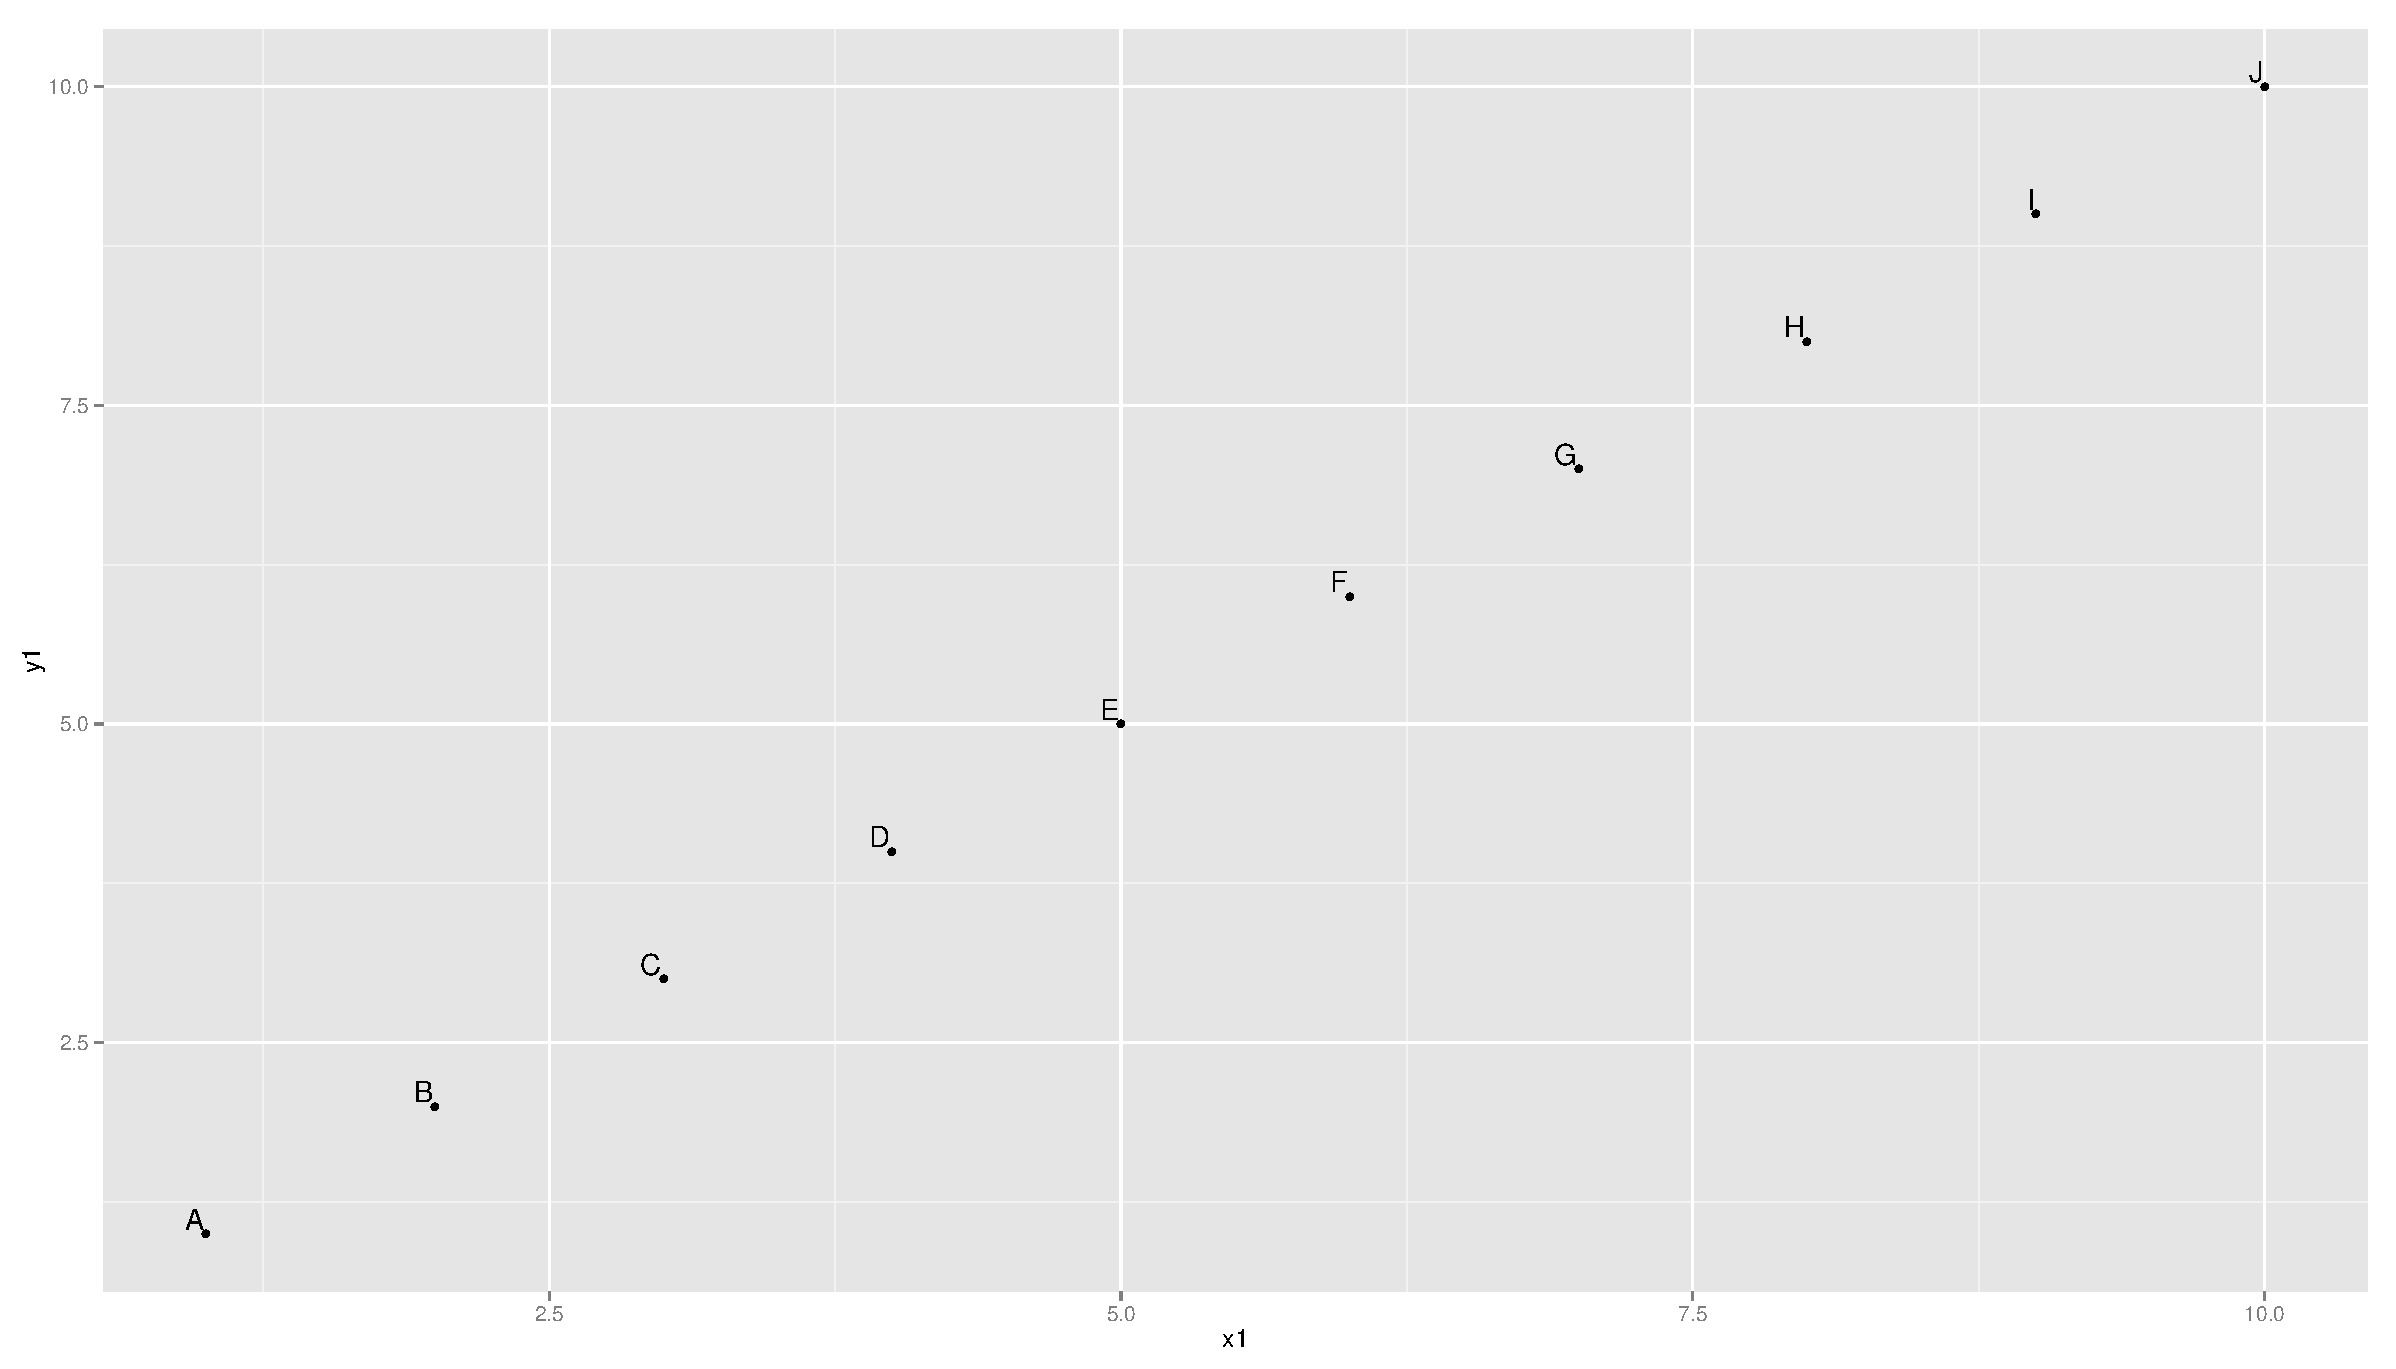
\includegraphics[width=3cm,height=3cm]{ggp2.pdf}}{ggp2.pdf}
\end{center}
\end{frame}


\begin{frame}[fragile]\frametitle{Layers}
  \begin{itemize}
  \item imagine you have worked a little time on a plot - and then you detect a mistake in your data, so the \emph{real} data frame looks different
  \item so you can replace the old, wrong data by the new  data (using \texttt{\%+\%} \footnotesize
\begin{verbatim}
> ## the new data
> ex2 <- data.frame(x1=sample(1:20),
+                   y1=sample(1:10),
+                   l=letters[1:20])
> head(ex2,10)
   x1 y1 l
1   3  6 a
2   6  2 b
3  14  1 c
4  19 10 d
5  12  4 e
6  15  8 f
7  20  5 g
8  17  7 h
9  13  3 i
10 16  9 j
\end{verbatim}
  \end{itemize}
\end{frame}


\begin{frame}[fragile]\frametitle{Layers}
\begin{verbatim}
> p2 %+% ex2
\end{verbatim}
\begin{center}
\linkimage{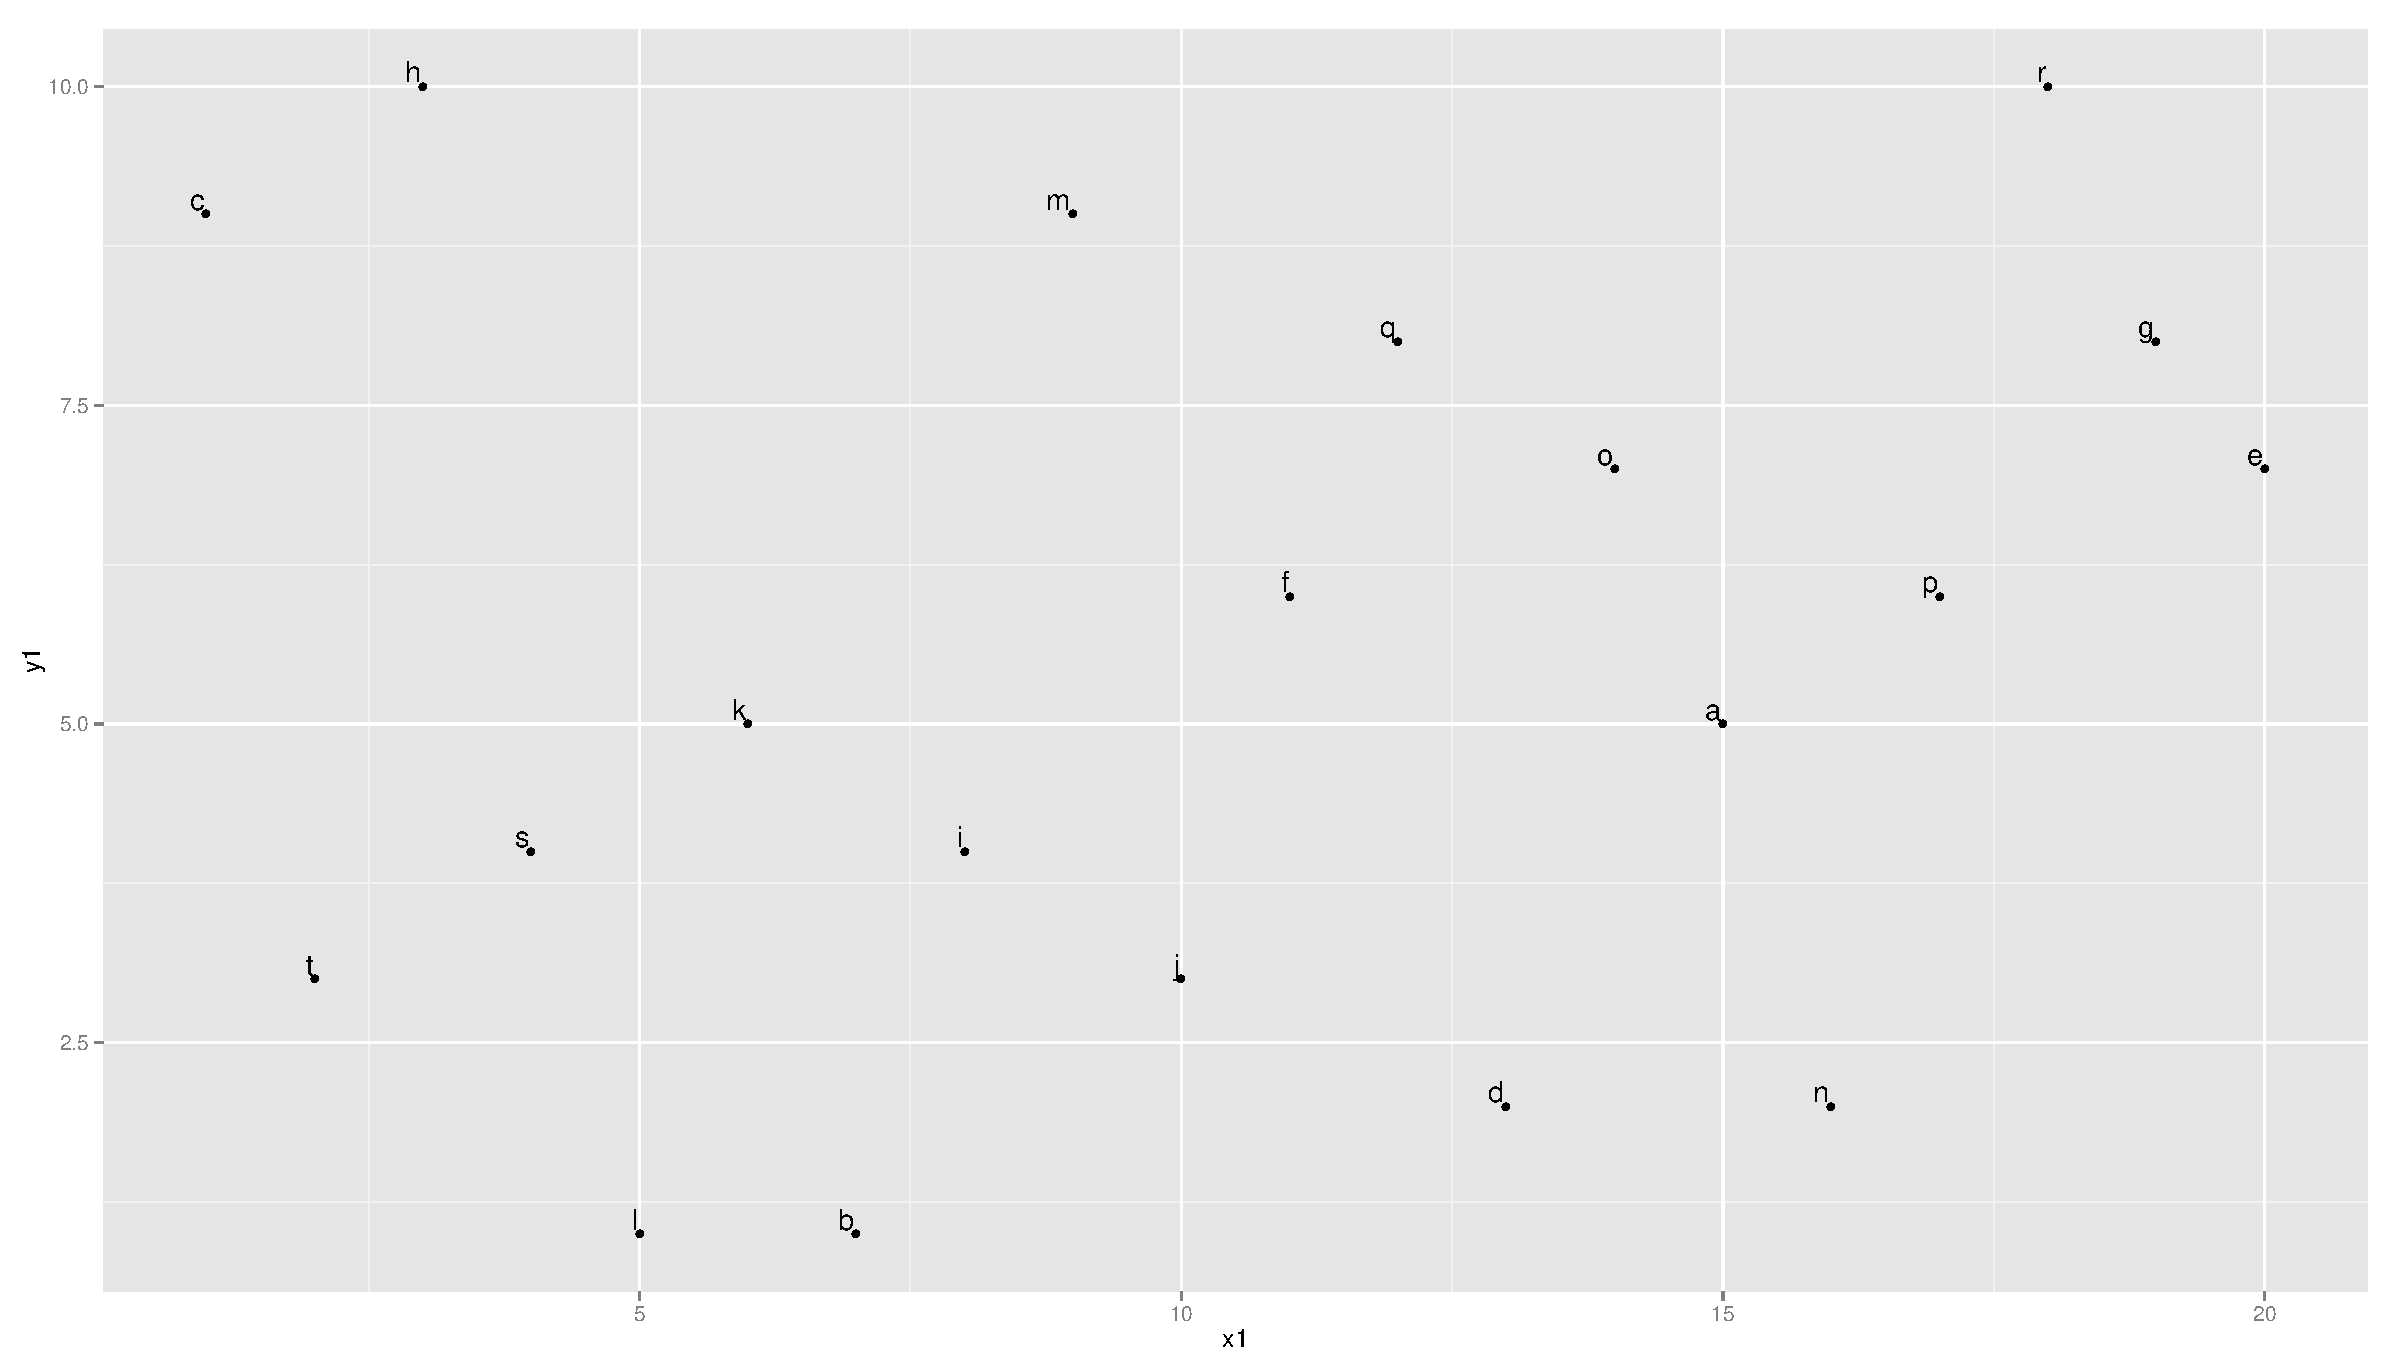
\includegraphics[width=3cm,height=3cm]{ggp3.pdf}}{ggp3.pdf}
\end{center}
\end{frame}

\begin{frame}[fragile]\frametitle{Layers}
  \begin{itemize}
  \item by using the line geom you can join the points (we use the new data)
\begin{verbatim}
> pn <- p %+% ex2 ## replace data in p
> pn + geom_line()
\end{verbatim}
  \end{itemize}
\begin{center}
\linkimage{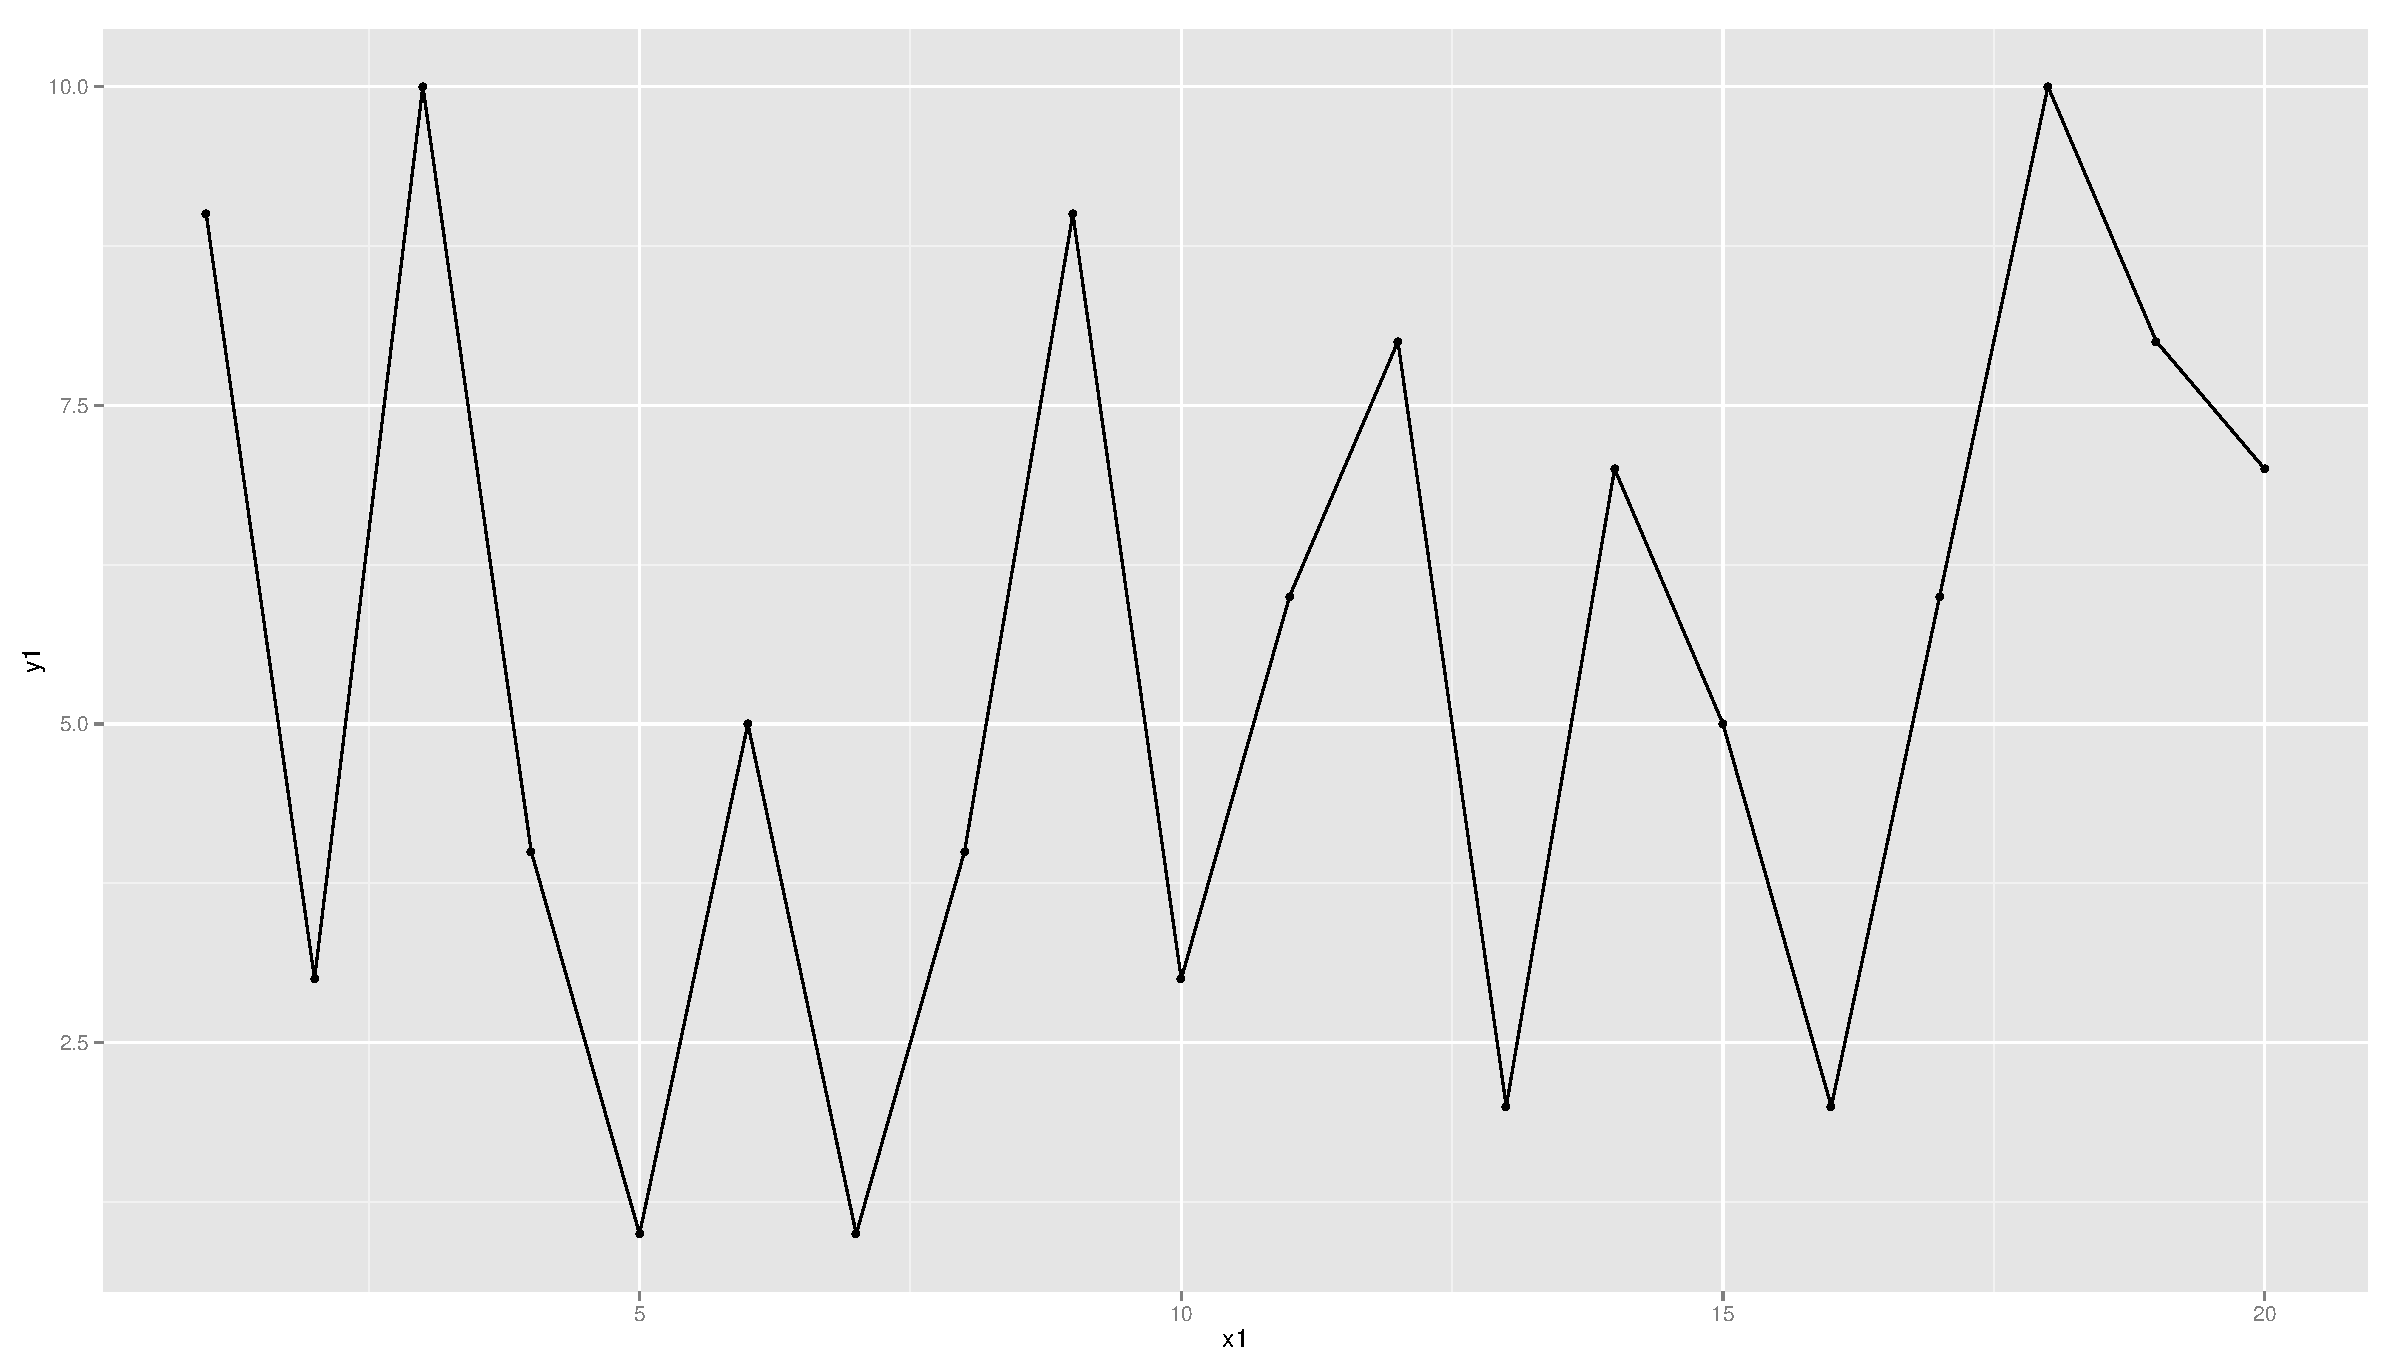
\includegraphics[width=3cm,height=3cm]{ggp4.pdf}}{ggp4.pdf}
\end{center}
\end{frame}

\begin{frame}[fragile]\frametitle{Layers}
  \begin{itemize}
  \item you can also join the points in the order of the data fram by using the path geom instead\footnotesize
\begin{verbatim}
> my.text <- geom_text(aes(label=l), 
+                          hjust=1.1, 
+                          vjust=-0.2)
> pn + geom_path() + my.text
\end{verbatim}
  \end{itemize}
\begin{center}
\linkimage{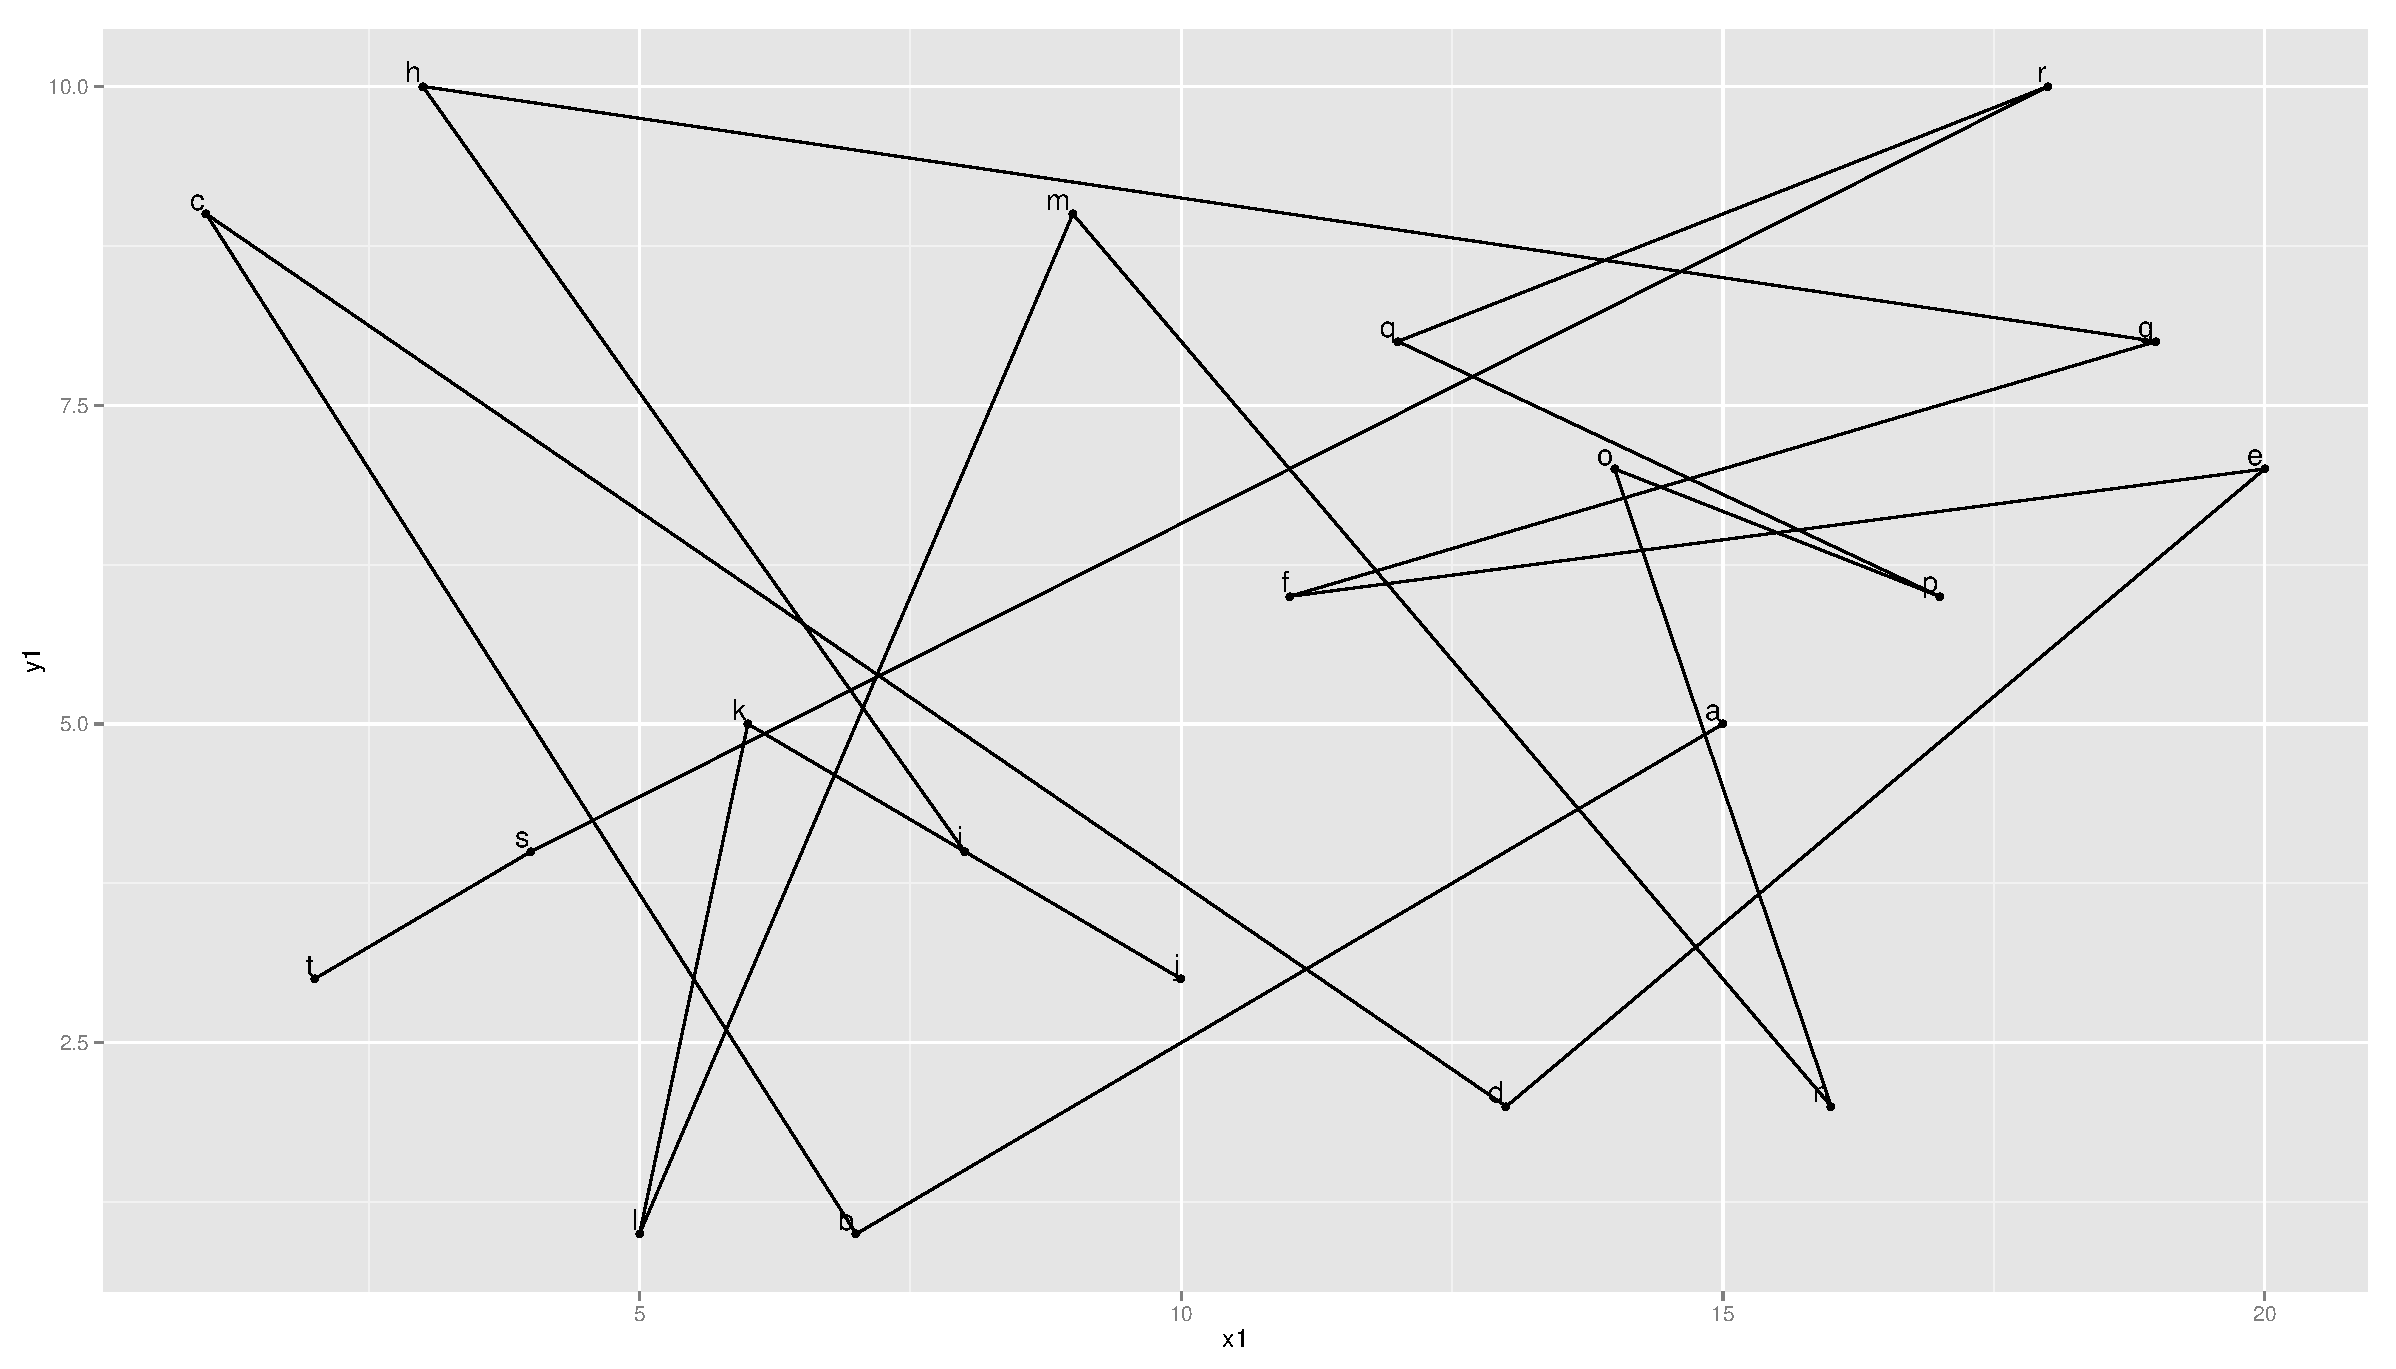
\includegraphics[width=3cm,height=3cm]{ggp5.pdf}}{ggp5.pdf}
\end{center}
\end{frame}

\begin{frame}[fragile]\frametitle{Layers}
Adding extra lines:
  \begin{itemize}
  \item there are three geoms: \texttt{abline, vline, hline}
  \item \texttt{abline} adds one or more lines with specified slope and intercept to the plot\footnotesize
\begin{verbatim}
> ## one line
> p + geom_abline(intercept=10,slope=-1,
+                          colour=rgb(.5,.5,.9))
> ## two lines
> p + geom_abline(intercept=c(10,9),slope=c(-1,-2),
+                              colour=rgb(.5,.5,.9))
> more lines
> p + geom_abline(intercept=10:1,slope=-(10:1)/10,
                                colour=rgb(.5,.5,.9))
\end{verbatim}
  \end{itemize}
\begin{center}
\linkimage{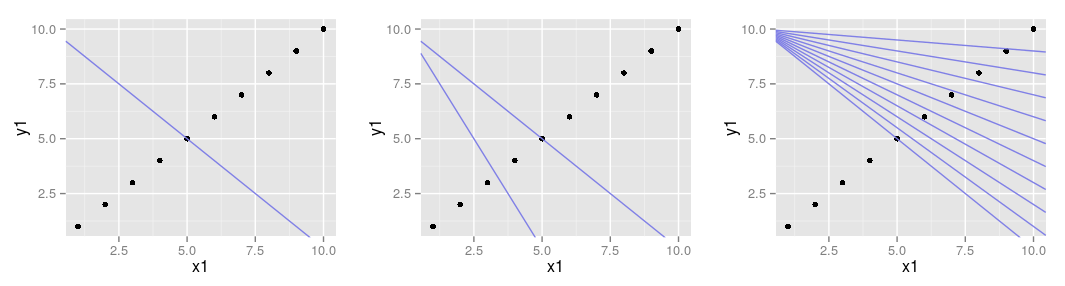
\includegraphics[width=5cm,height=2.5cm]{ggp6.png}}{ggp6.png}
\end{center}
\end{frame}

\begin{frame}[fragile]\frametitle{Layers}
  \begin{itemize}
  \item adding lines referring to the data frame
\begin{verbatim}
> p1 +
+   geom_abline(aes(slope=b,intercept=a,colour=x1)) + 
+   scale_x_continuous(limits=c(0,10)) 
\end{verbatim}
  \end{itemize}
\begin{center}
\linkimage{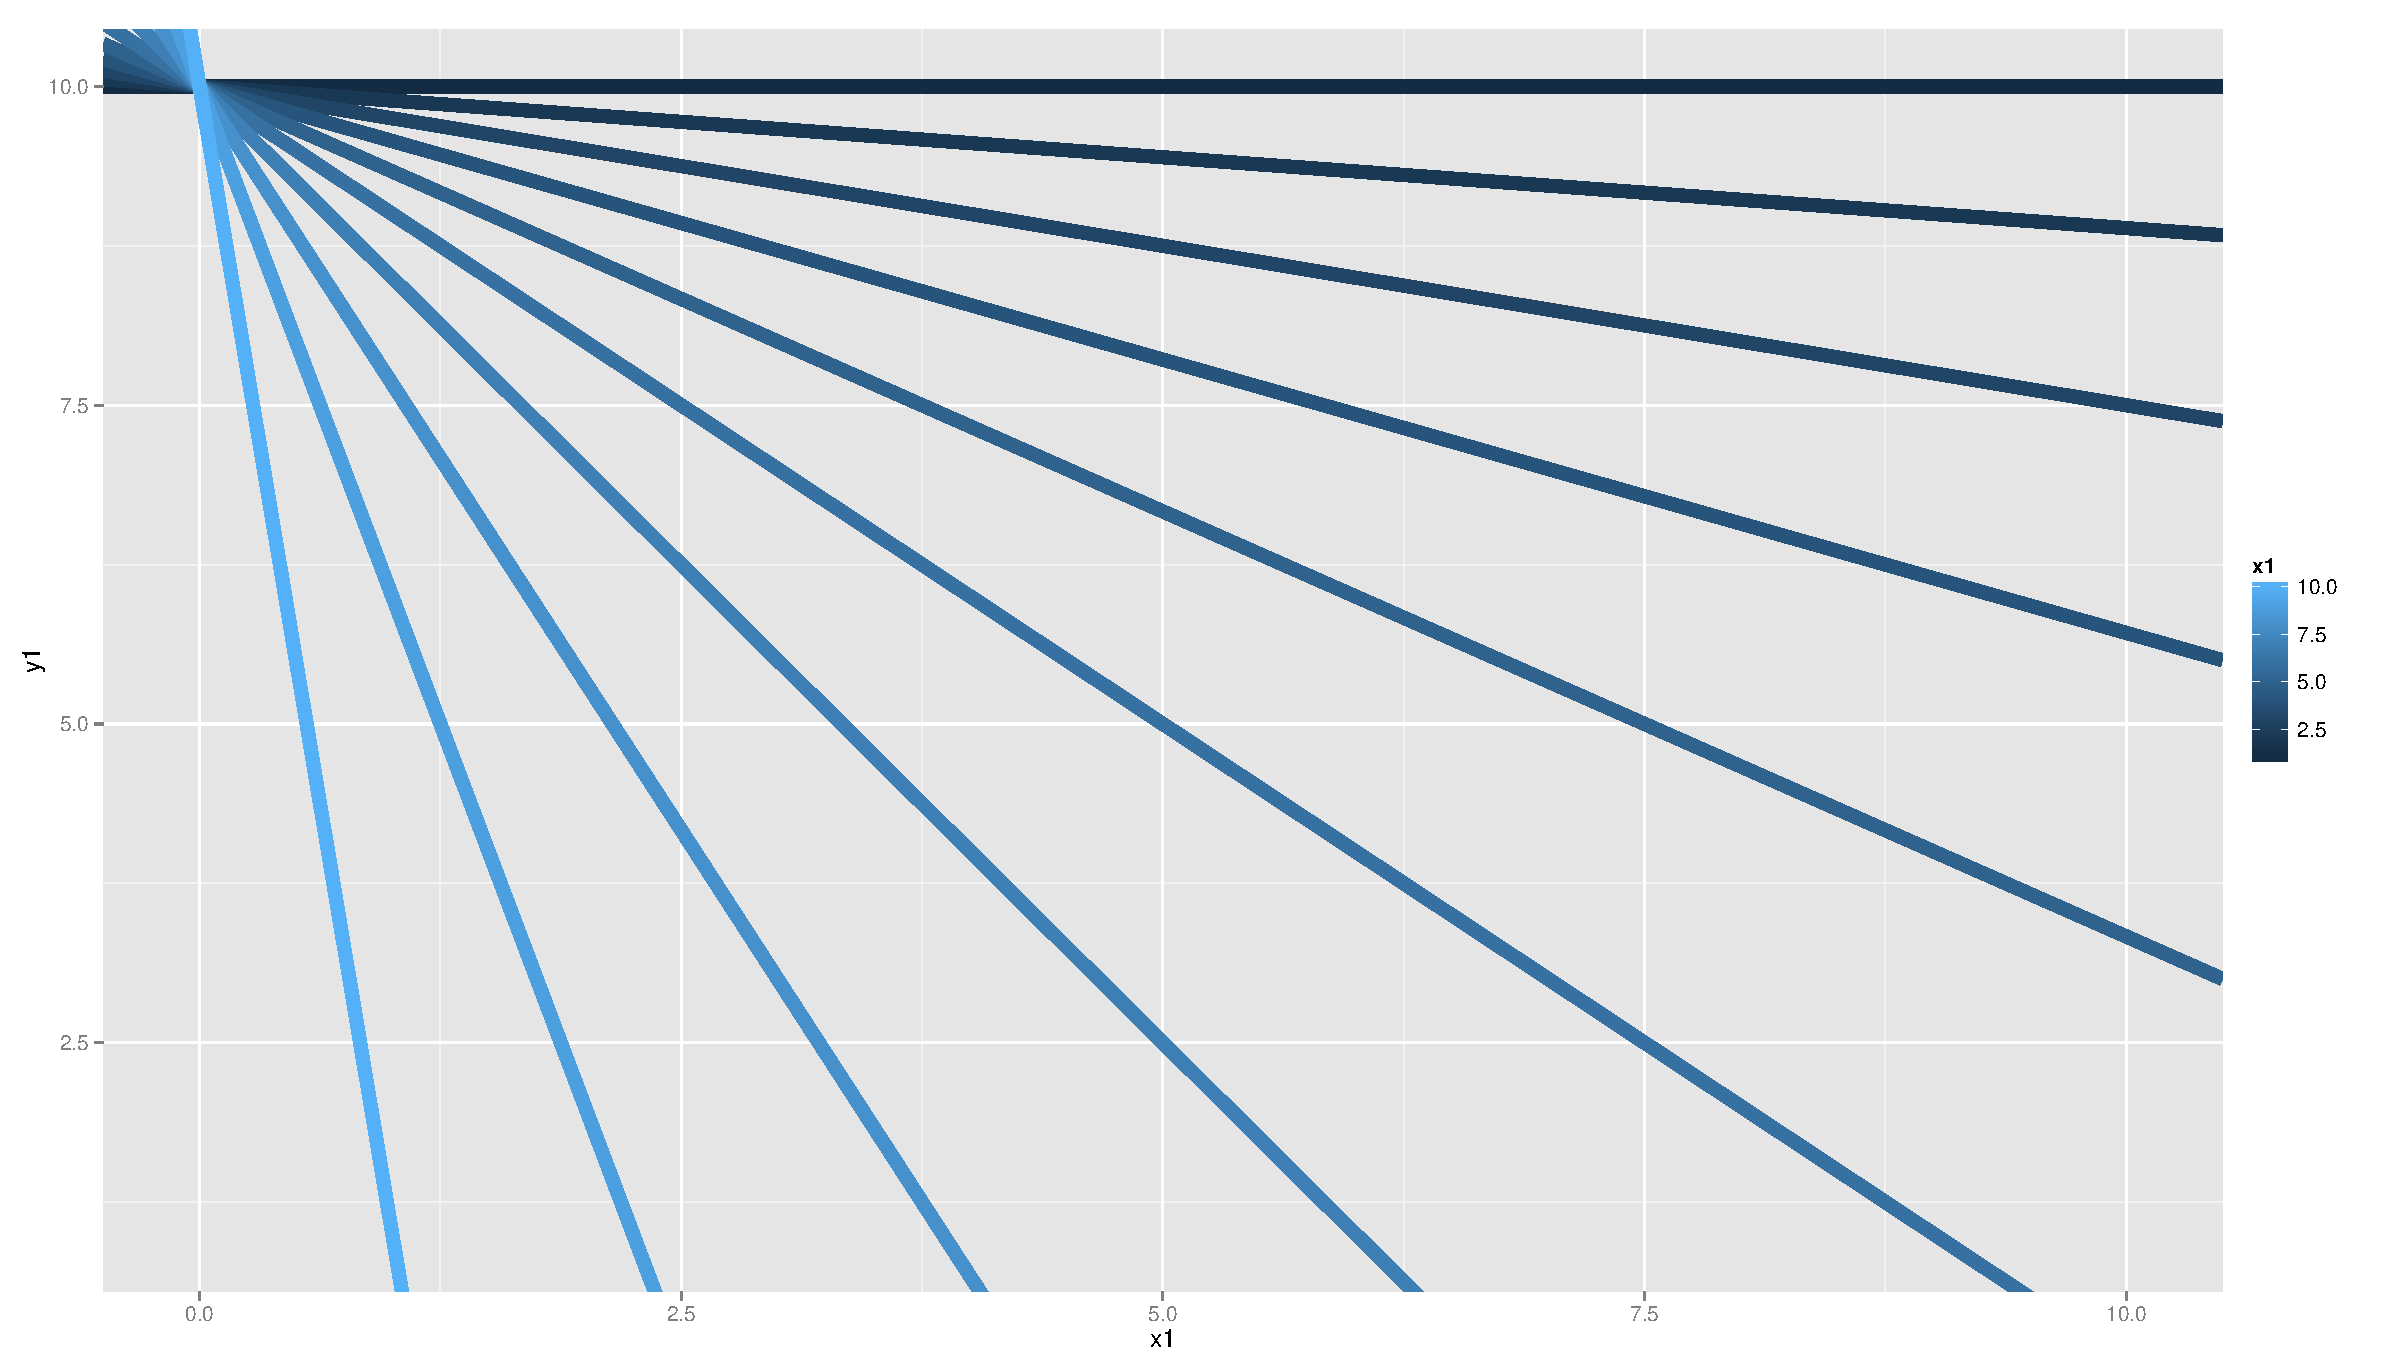
\includegraphics[width=3cm,height=3cm]{ggp7.pdf}}{ggp7.pdf}
\end{center}
\end{frame}

\begin{frame}[fragile]\frametitle{Layers}
  \begin{itemize}
  \item the same works for the hline and the vline geom which add horizonal and vertical line(s)
  \item argument: yintercept, xintercept respectively
  \item setting and mapping are possible
\begin{verbatim}
> p1 + geom_hline(yintercept=1:10)
> p1 + geom_hline(yintercept=1:10) + 
+     geom_vline(xintercept=1:10)
\end{verbatim}
  \end{itemize}
\begin{center}
\linkimage{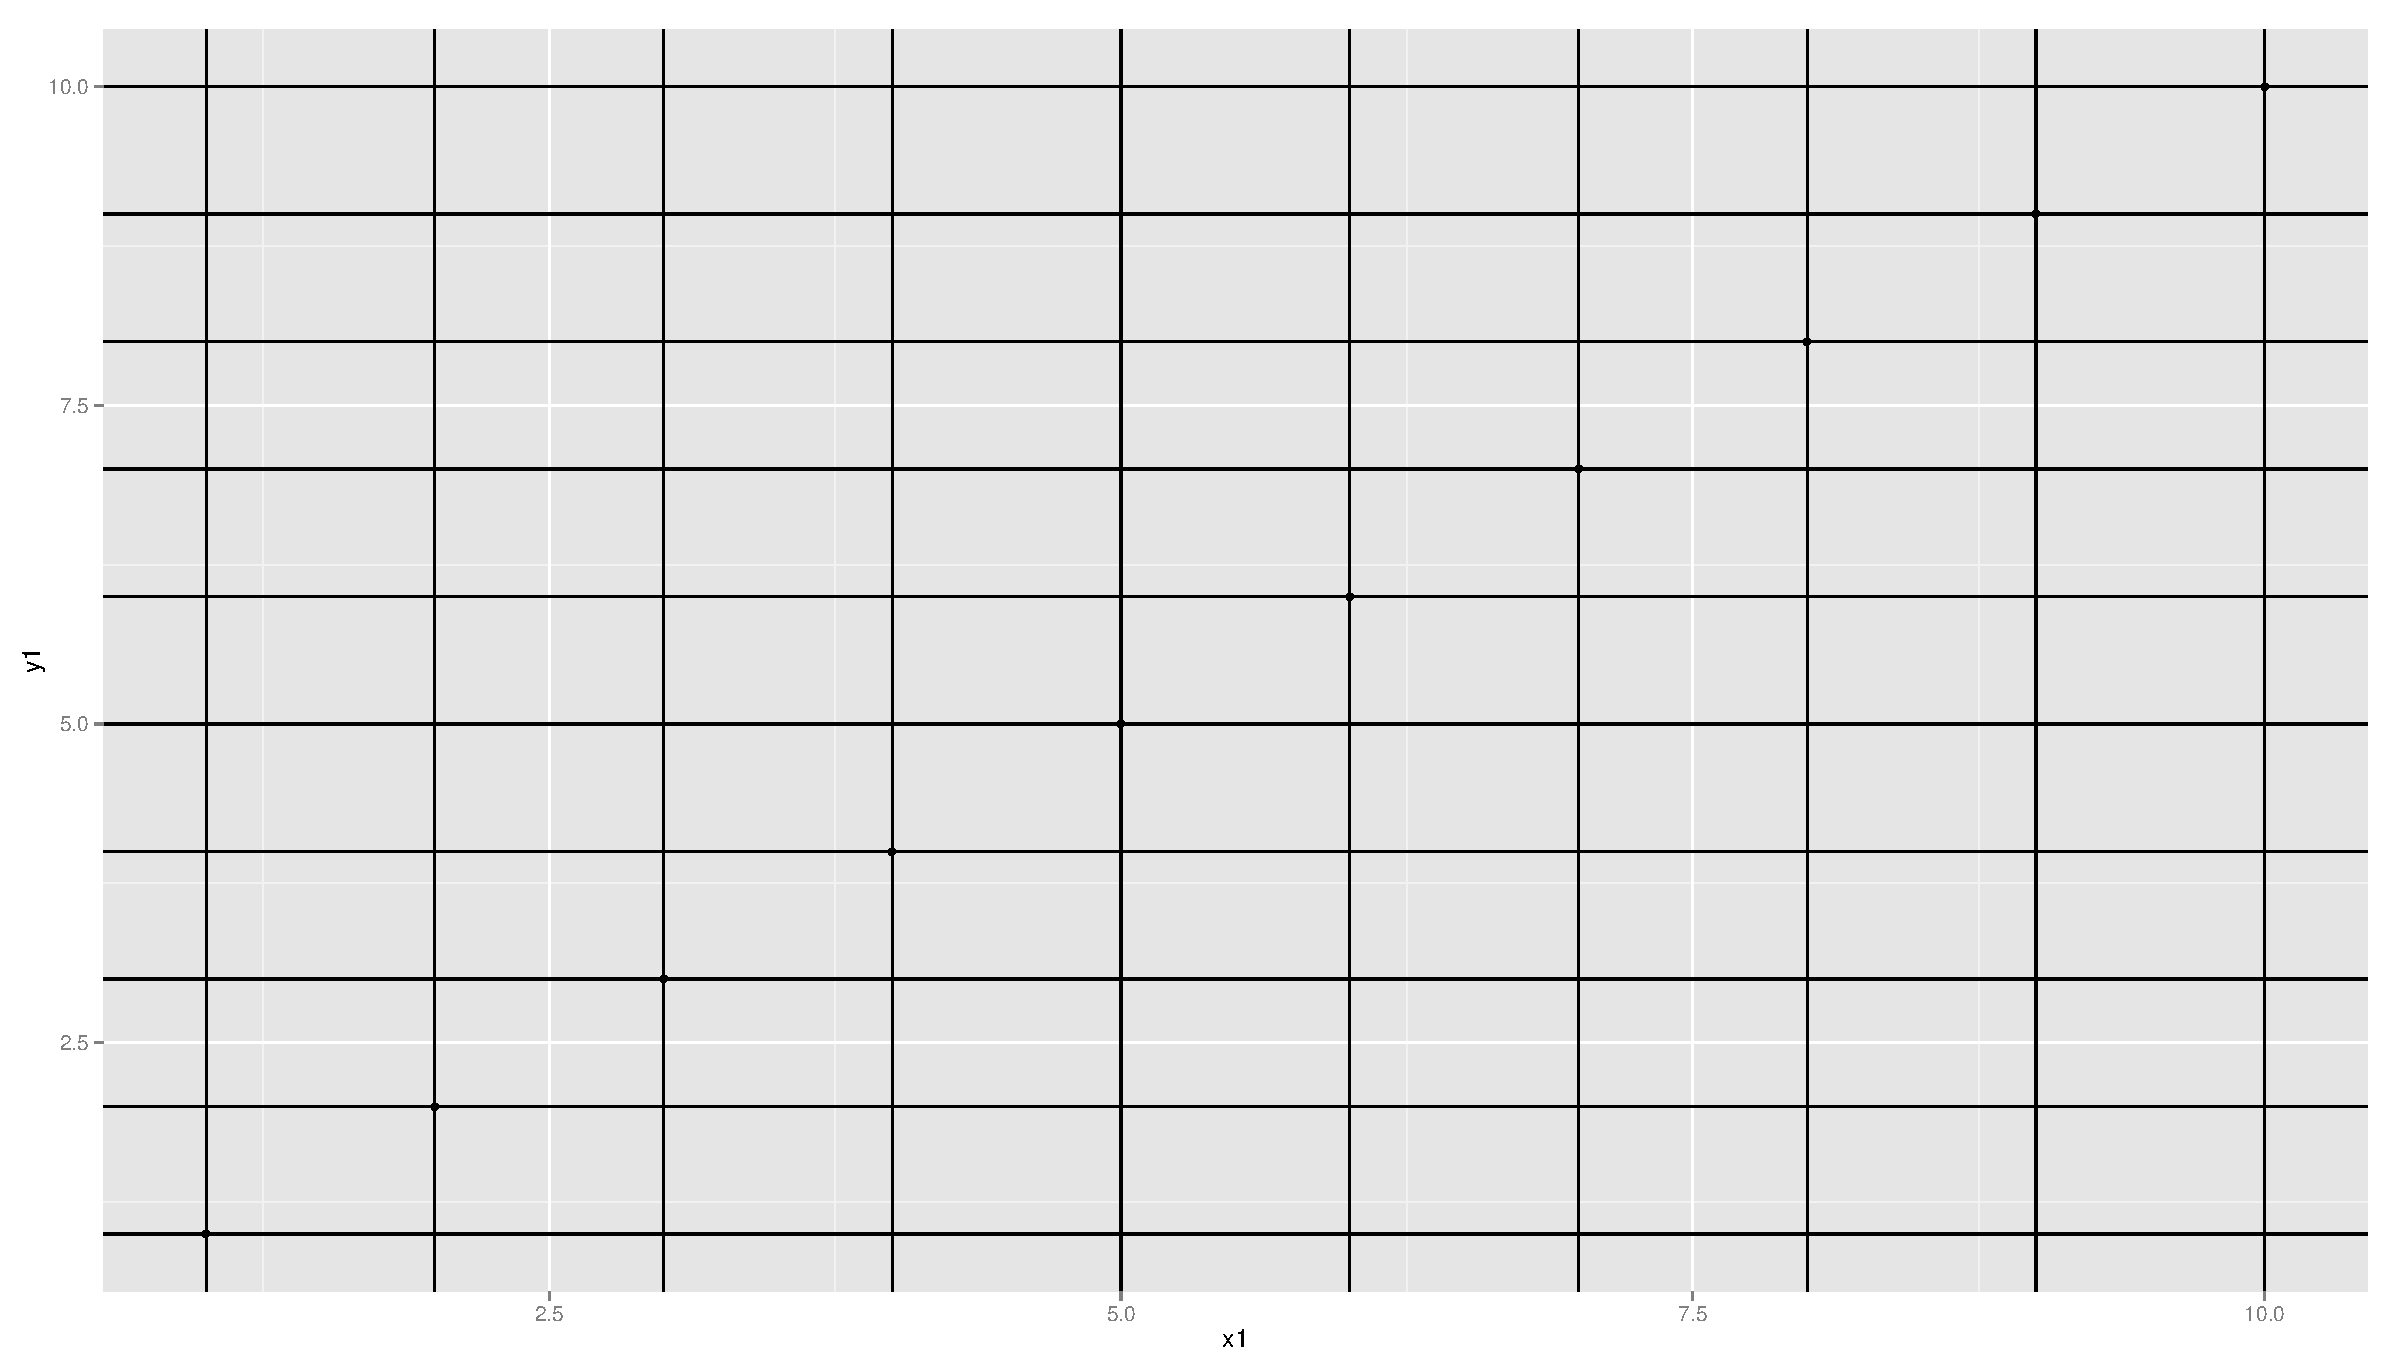
\includegraphics[width=3cm,height=3cm]{ggp8.pdf}}{ggp8.pdf}
\end{center}
\end{frame}

\begin{frame}[fragile]\frametitle{Other Common Layers}
\begin{itemize}
\item some other layers for 1 continuous variable:
  \begin{itemize}
  \item \texttt{geom\_boxplot()}
  \item \texttt{geom\_histogram()}
  \item \texttt{geom\_density()}
  \end{itemize}
\item some other layers for 1 discrete variable:
  \begin{itemize}
  \item \texttt{geom\_bar()}
  \end{itemize}
\item some other layers for 2 or more continuous variables:
  \begin{itemize}
  \item \texttt{geom\_smooth()}
  \item \texttt{geom\_density2d()}
  \item \texttt{geom\_contour()}
  \item \texttt{geom\_quantile()}
  \end{itemize}
\end{itemize}
\end{frame}

\subsection{Exercises I}
\begin{frame}[fragile]\frametitle{Exercises}
  \begin{itemize}
  \item use our data frame or load it (file "201503data.rdata)
  \item create a new variable EC1 containing the first 2 letters of the Event.Code column, use the function \texttt{str\_sub()} from the stringr package (type \texttt{?str\_sub}  to get help)
  \end{itemize}
\end{frame}


\begin{frame}[fragile]\frametitle{Exercises}\tiny
\begin{verbatim}
> data$EC1 <- factor(str_sub(data$Event.Code,1,2))
> head(data)
  Subject Sex Age_PRETEST Trial Event.Type Code   Time TTime Uncertainty
1       1   f        3.11     7   Response    2 103745  2575           1
2       1   f        3.11    12   Response    2 156493  2737           1
3       1   f        3.11    17   Response    2 214772  6630           1
4       1   f        3.11    22   Response    1 262086  5957           1
5       1   f        3.11    27   Response    2 302589   272           1
6       1   f        3.11    32   Response    1 352703  7197           1
  Duration Uncertainty.1 ReqTime ReqDur Stim.Type Pair.Index    Type Event.Code
1     2599             3       0   next       hit          7 Picture   RO26.jpg
2     2800             2       0   next incorrect         12 Picture   RO19.jpg
3     6798             2       0   next       hit         17 Picture   RS23.jpg
4     5999             2       0   next incorrect         22 Picture   OF22.jpg
5      400             2       0   next       hit         27 Picture   AT08.jpg
6     7398             2       0   next       hit         32 Picture   AT30.jpg
  testid EC1
1  test2  RO
2  test2  RO
3  test2  RS
4  test2  OF
5  test2  AT
6  test2  AT
\end{verbatim}
\end{frame}

\begin{frame}[fragile]\frametitle{Exercises}
Create the six plots and save them into a file.
  \begin{enumerate}
  \item create a plot using ggplot, map the variable EC1 to x and use \texttt{geom\_bar()}
  \item now to the plot again, but add another aesthetic: \texttt{fill} (colour of the filling); map \texttt{fill} to \texttt{Stim.Type}
  \item add the \texttt{position} argument to \texttt{geom\_bar()}, set it to "fill"
  \item now add \texttt{facet\_wrap(~testid)} to show the same graph per time
  \item make a graph facetted per child showing stacked hit/incorrect bars with time on the x axis
  \item show the distribution of the variable \texttt{TTime} using \texttt{geom\_boxplot()} again facetted per child and separated per hit/incorrect
  \end{enumerate}
\end{frame}


\begin{frame}[fragile]\frametitle{Exercises}
  \begin{itemize}
  \item create a plot using ggplot, map the variable EC1 to x and use \texttt{geom\_bar()}
  \end{itemize}
\begin{verbatim}
> ggplot(data,aes(x=EC1)) +
+     geom_bar()
> 
> ggsave("plot1.png")
Saving 16 x 9.13 in image  
\end{verbatim}
\begin{center}
\linkimage{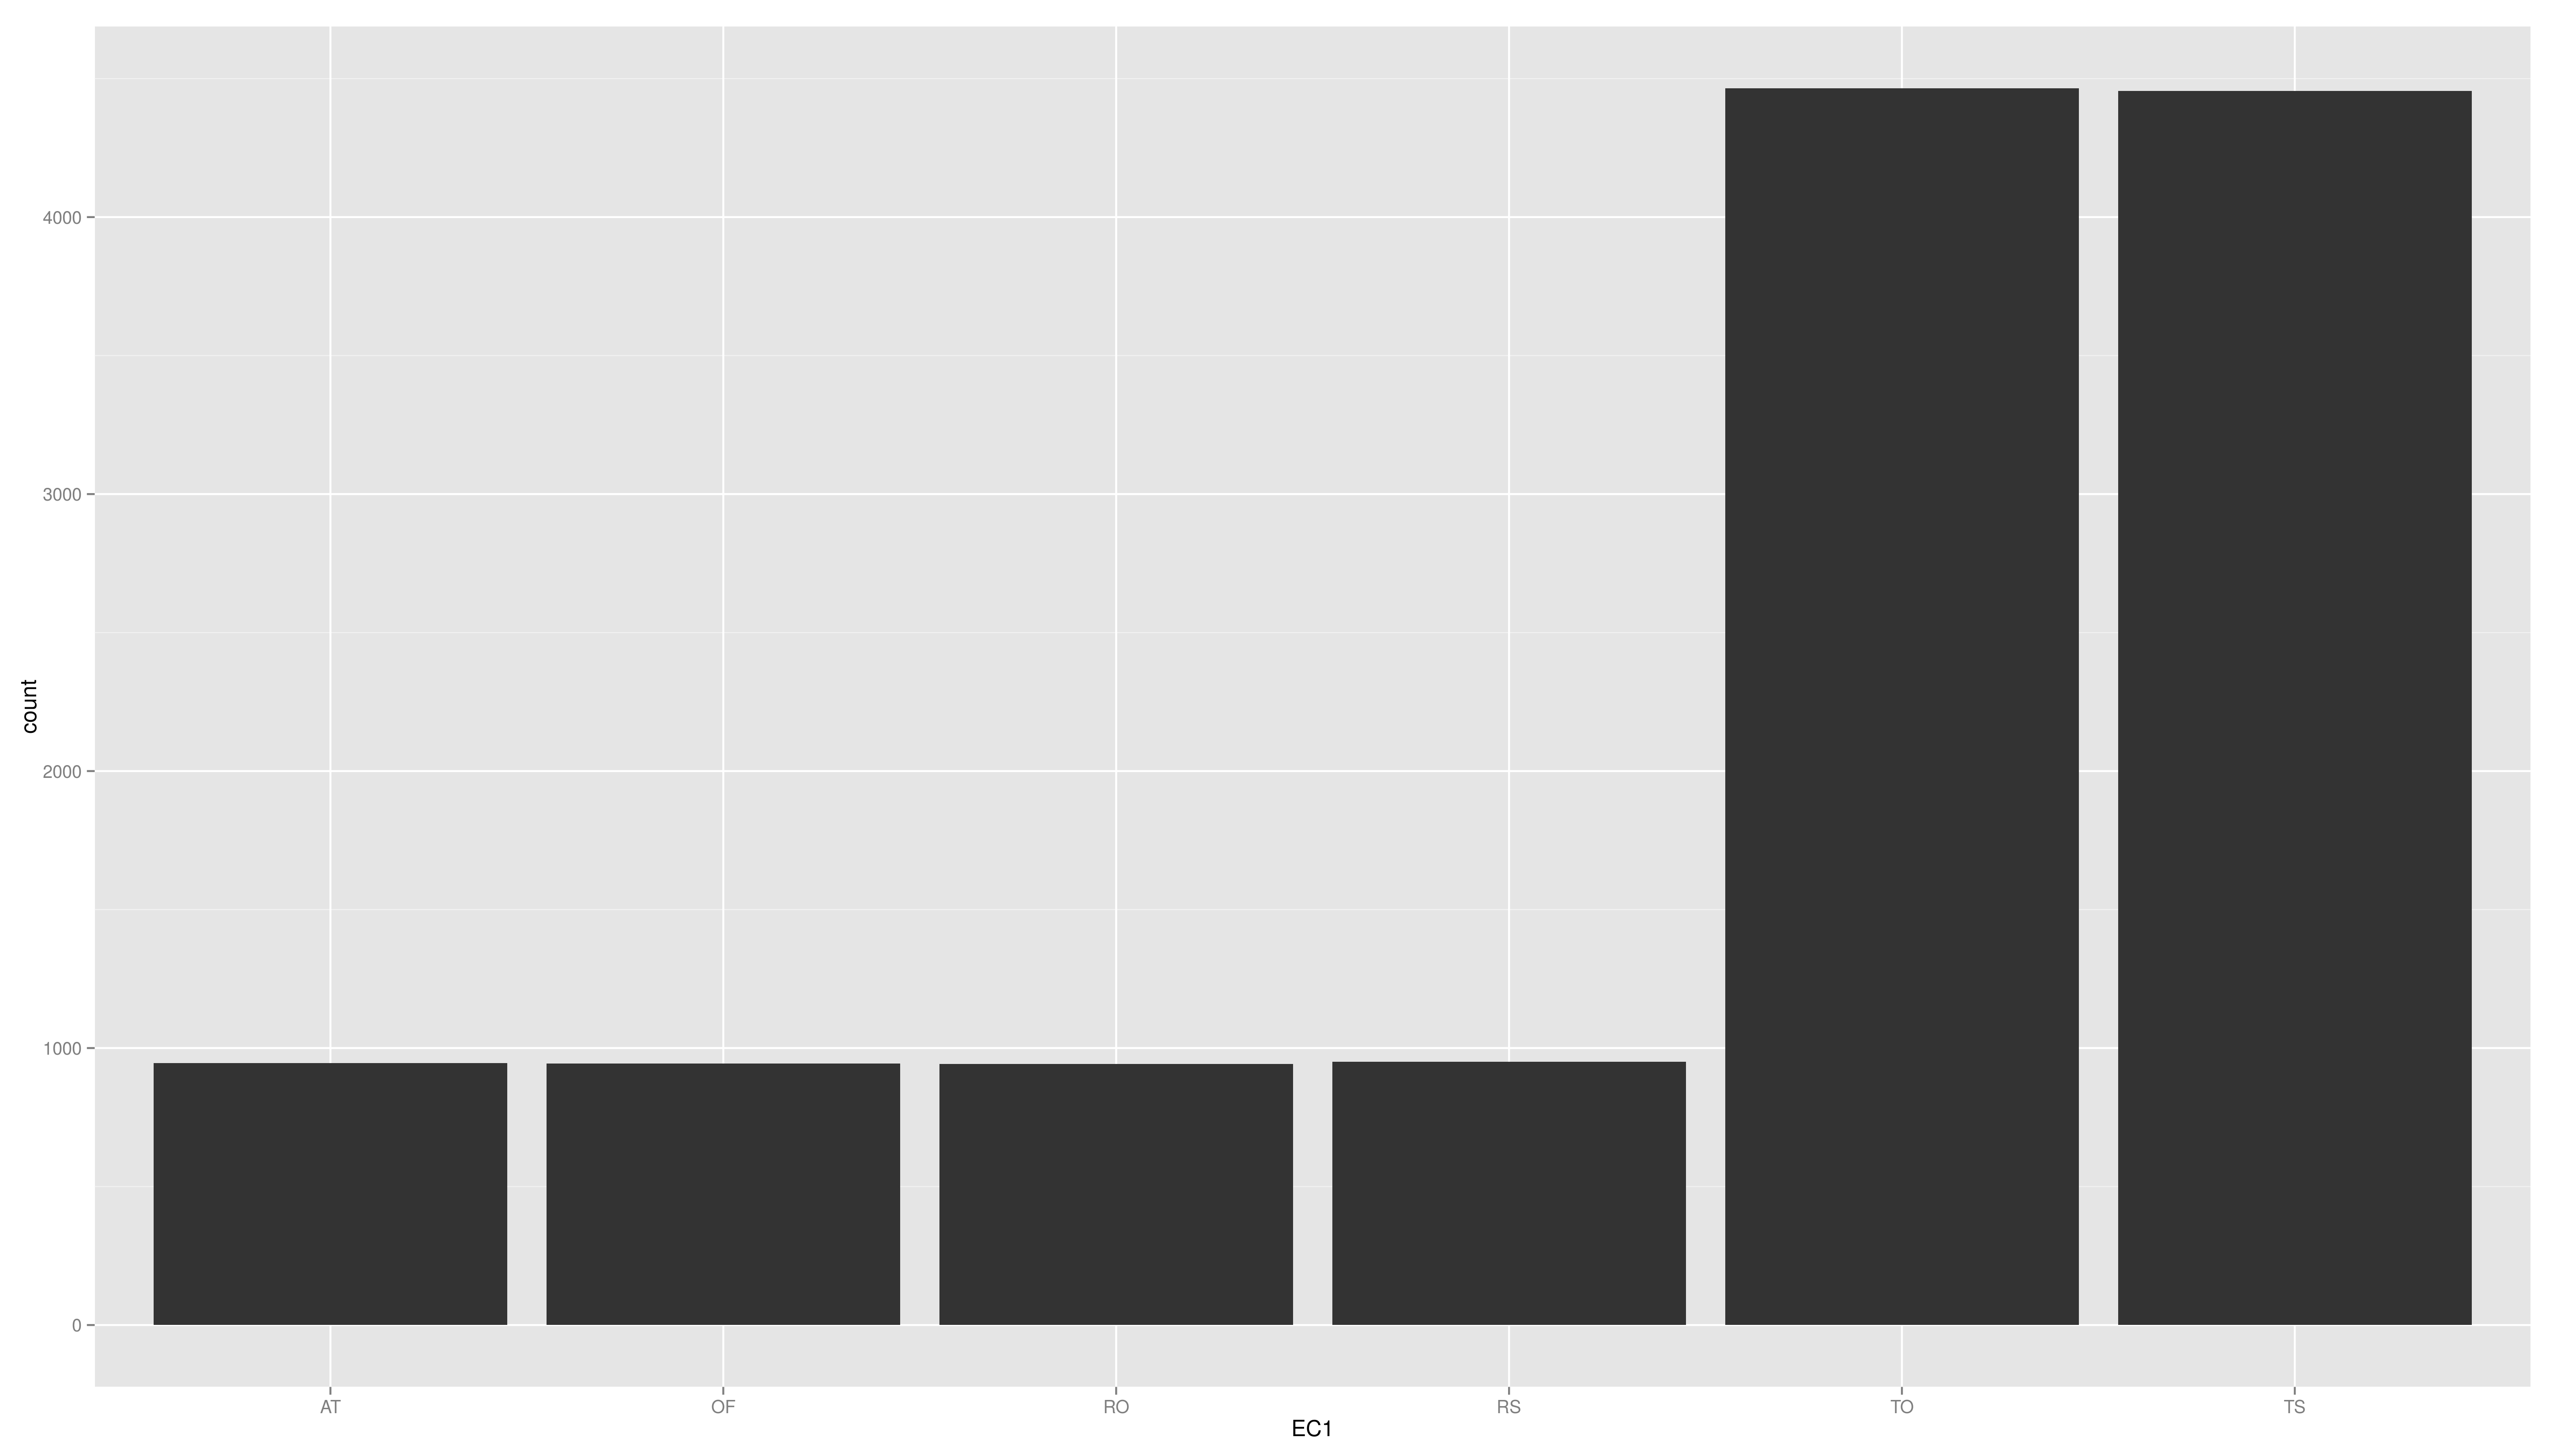
\includegraphics[width=3cm,height=3cm]{plot1.png}}{plot1.png}
\end{center}
\end{frame}


\begin{frame}[fragile]\frametitle{Exercises}
  \begin{itemize}
  \item now to the plot again, but add another aesthetic: \texttt{fill} (colour of the filling); map \texttt{fill} to \texttt{Stim.Type}
  \end{itemize}
\begin{verbatim}
> ggplot(data,aes(x=EC1,fill=Stim.Type)) +
+     geom_bar()
> 
> ggsave("plot2.png")
Saving 16 x 9.13 in image
\end{verbatim}
\begin{center}
\linkimage{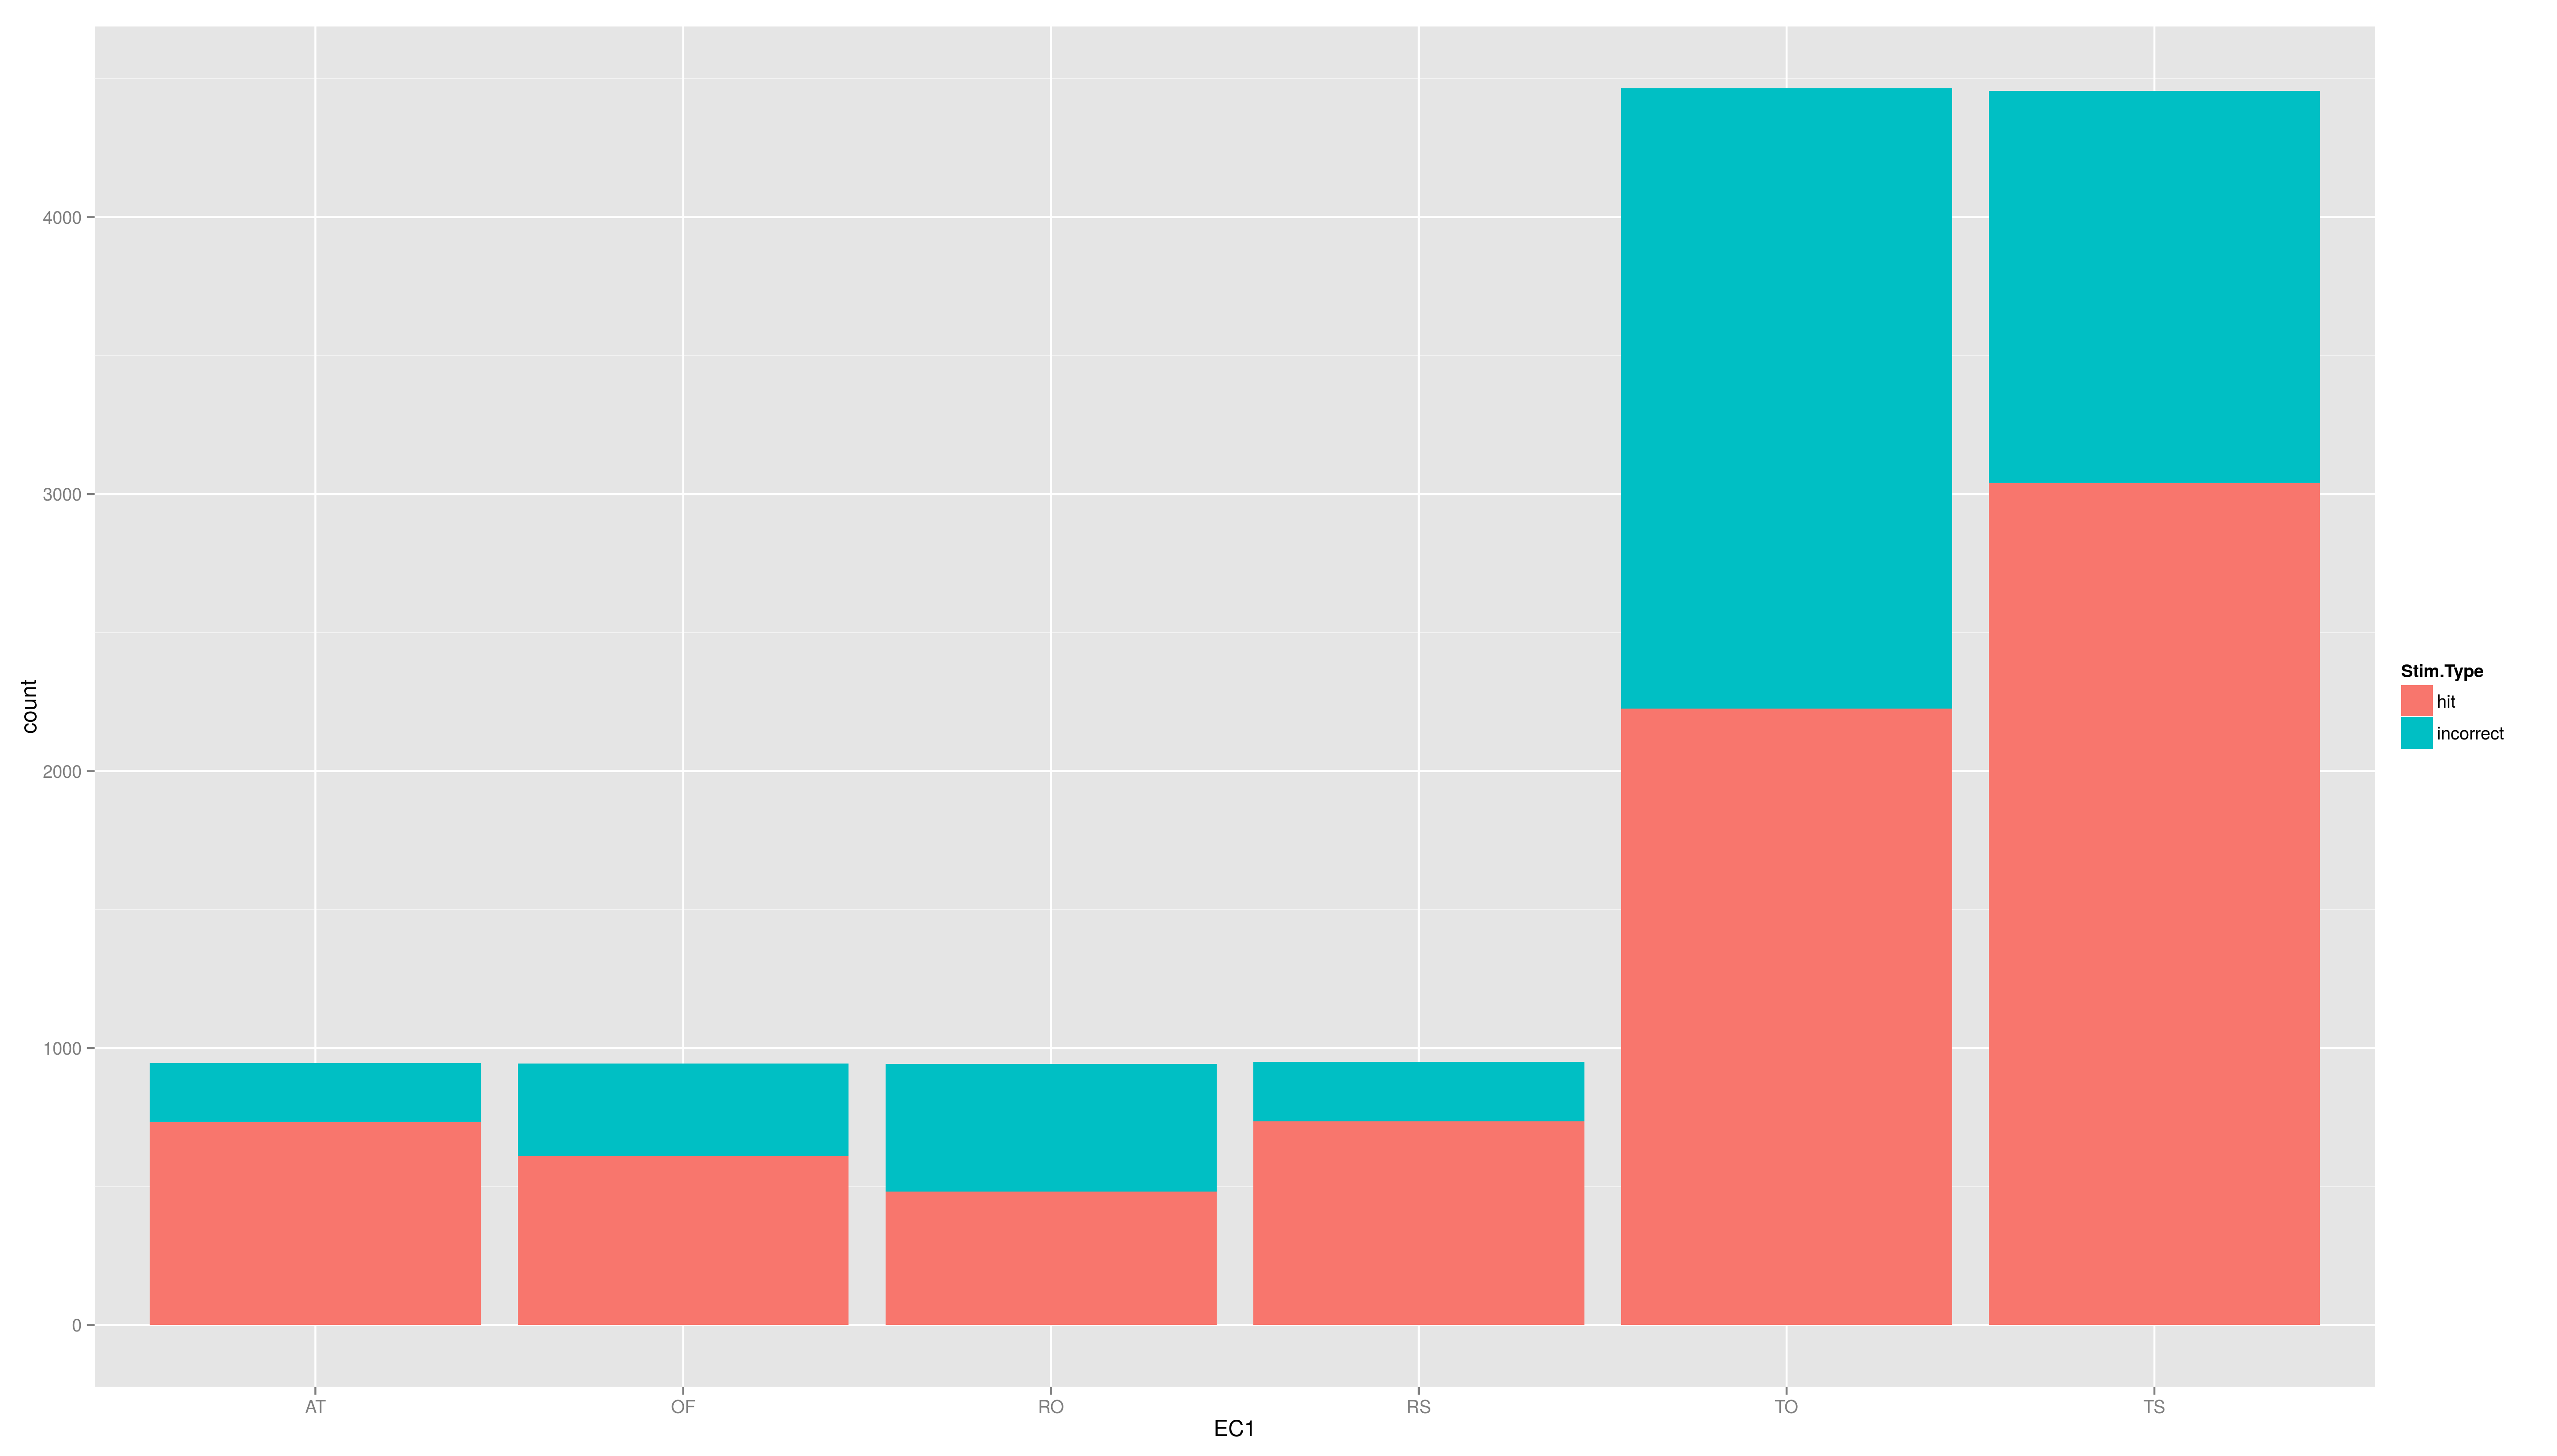
\includegraphics[width=3cm,height=3cm]{plot2.png}}{plot2.png}
\end{center}
\end{frame}

\begin{frame}[fragile]\frametitle{Exercises}
  \begin{itemize}
  \item add the \texttt{position} argument to \texttt{geom\_bar()}, set it to "fill"
  \end{itemize}
\begin{verbatim}
> ggplot(data,aes(x=EC1,fill=Stim.Type)) +
+     geom_bar(position = "fill")
> 
> ggsave("plot3.png")
Saving 16 x 9.13 in image
\end{verbatim}
\begin{center}
\linkimage{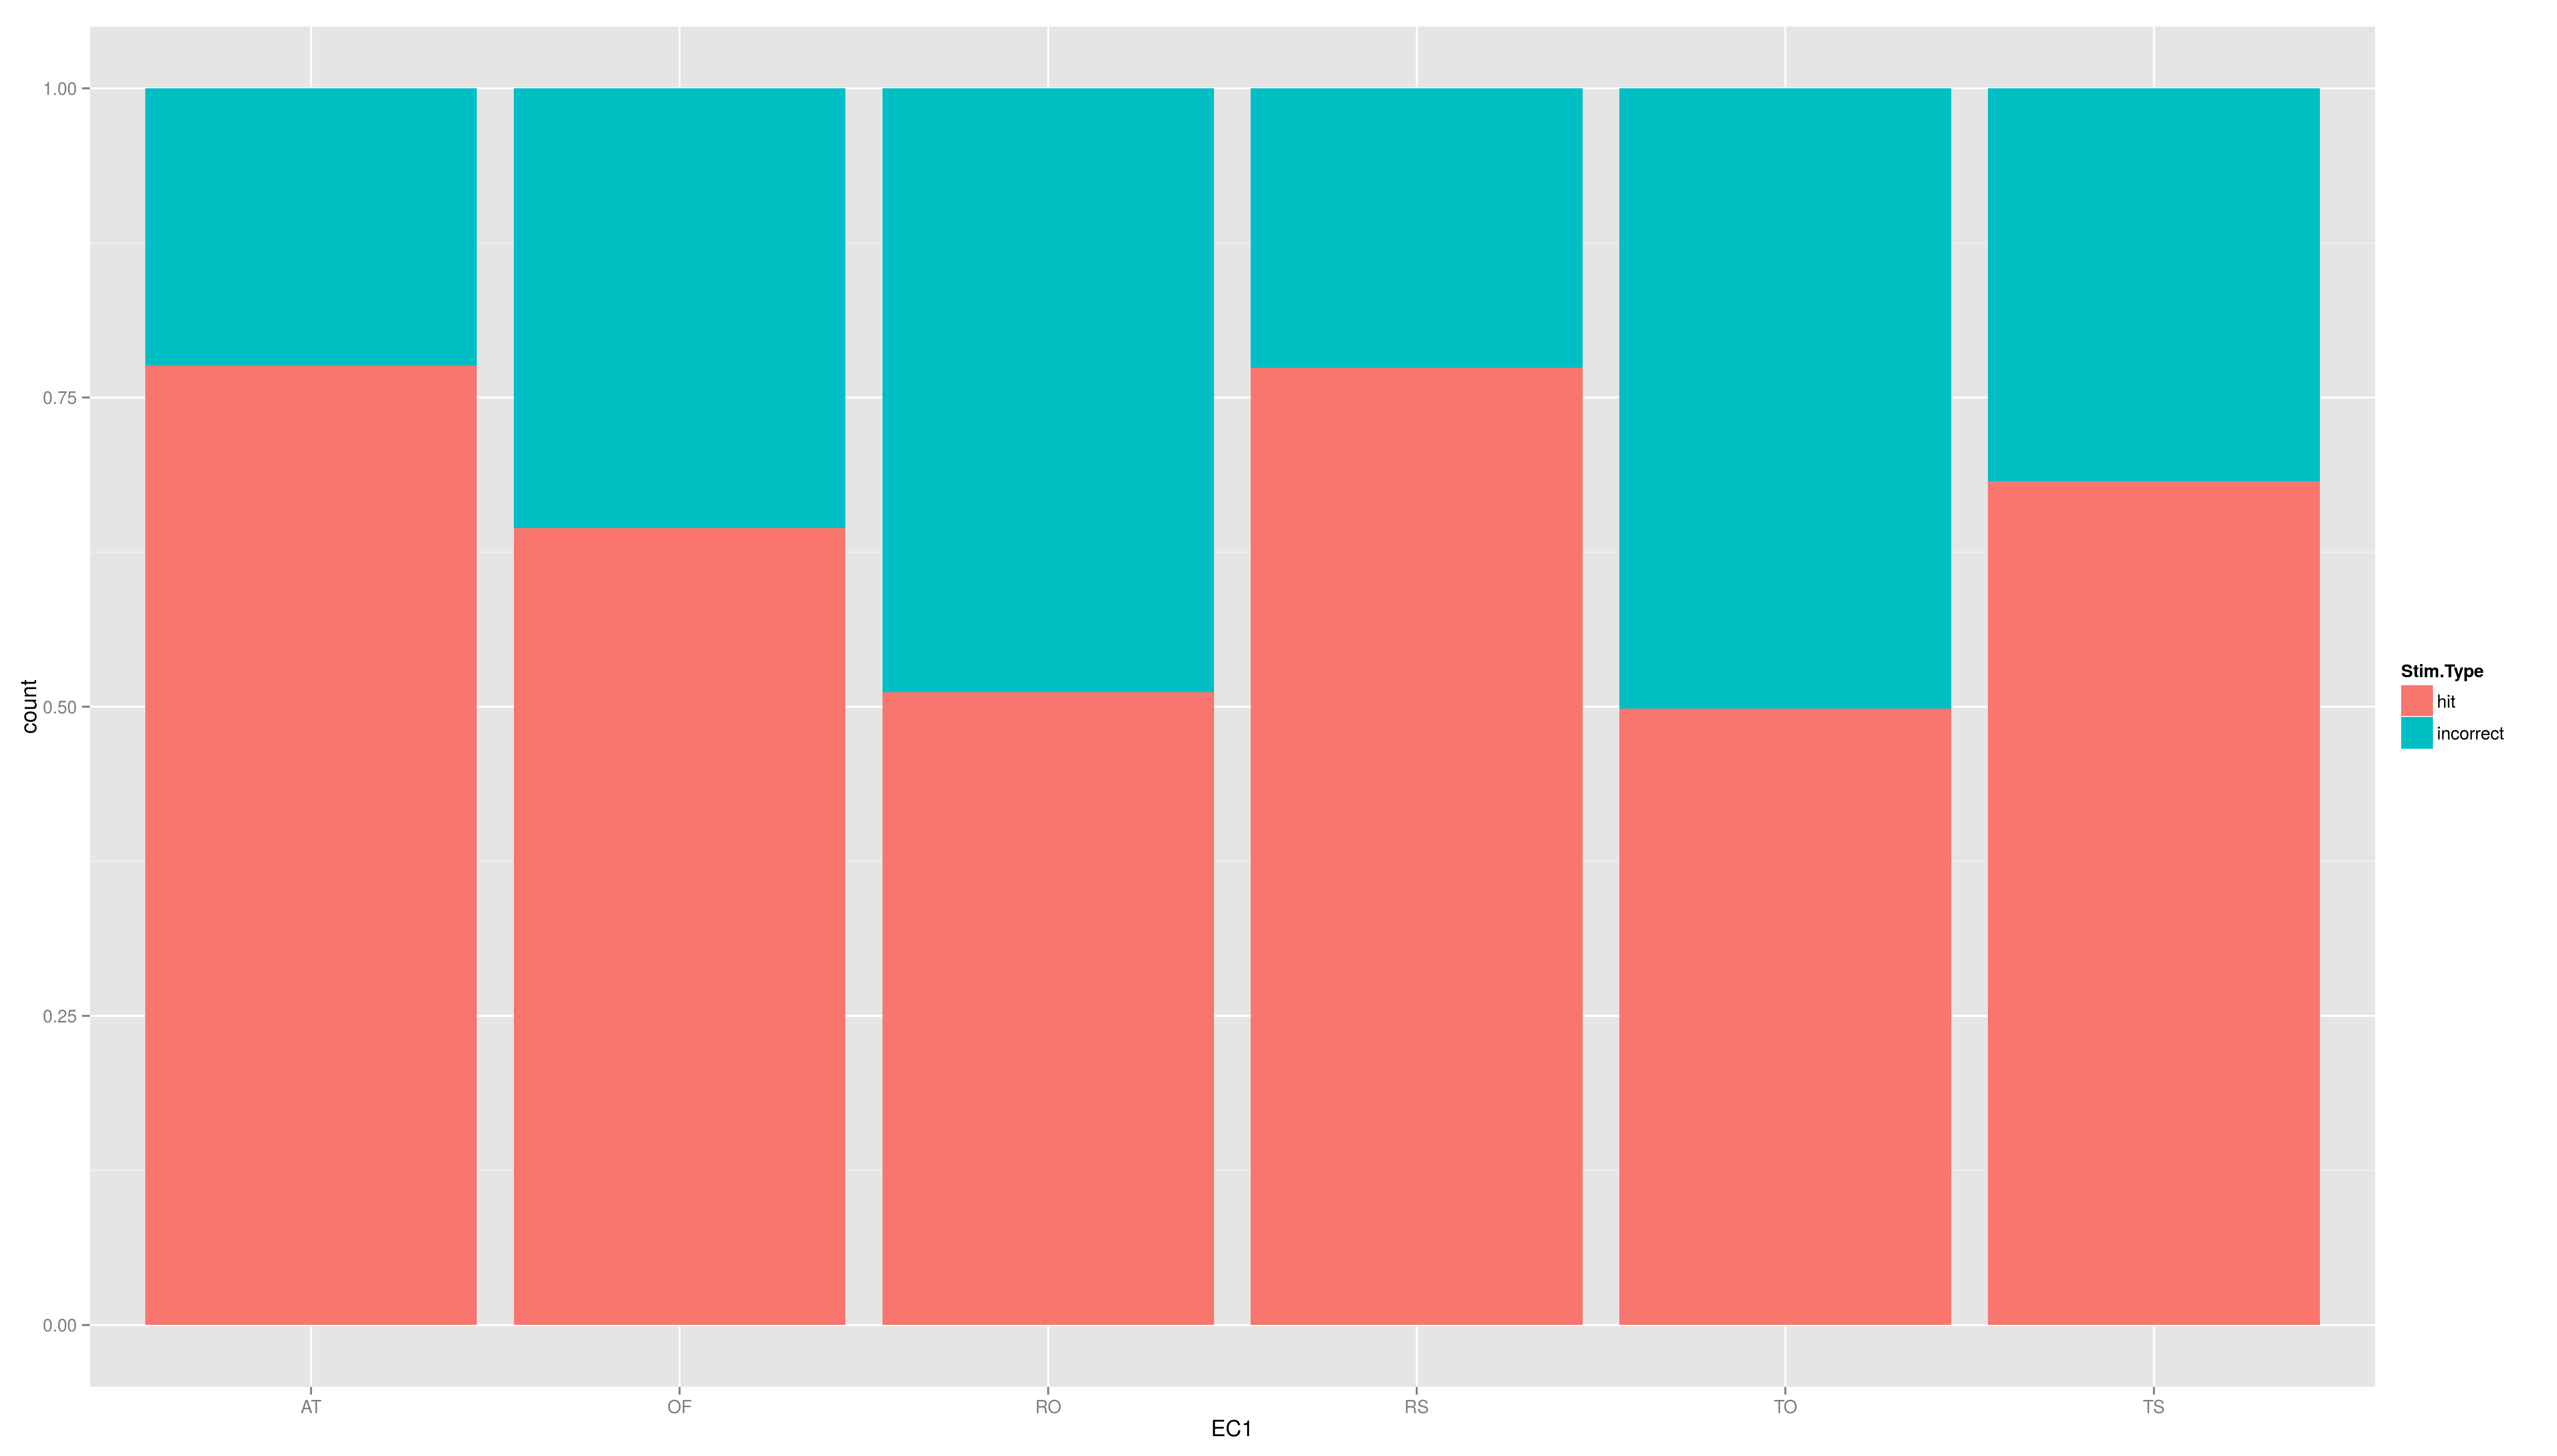
\includegraphics[width=3cm,height=3cm]{plot3.png}}{plot3.png}
\end{center}
\end{frame}


\begin{frame}[fragile]\frametitle{Exercises}
  \begin{itemize}
  \item now add \texttt{facet\_wrap(~testid)} to show the same graph per time
  \end{itemize}
\begin{verbatim}
> ggplot(data,aes(x=EC1,fill=Stim.Type)) +
+     geom_bar(position = "fill") +
+     facet_wrap(~testid)
> 
> ggsave("plot4.png")
Saving 16 x 9.13 in image
\end{verbatim}
\begin{center}
\linkimage{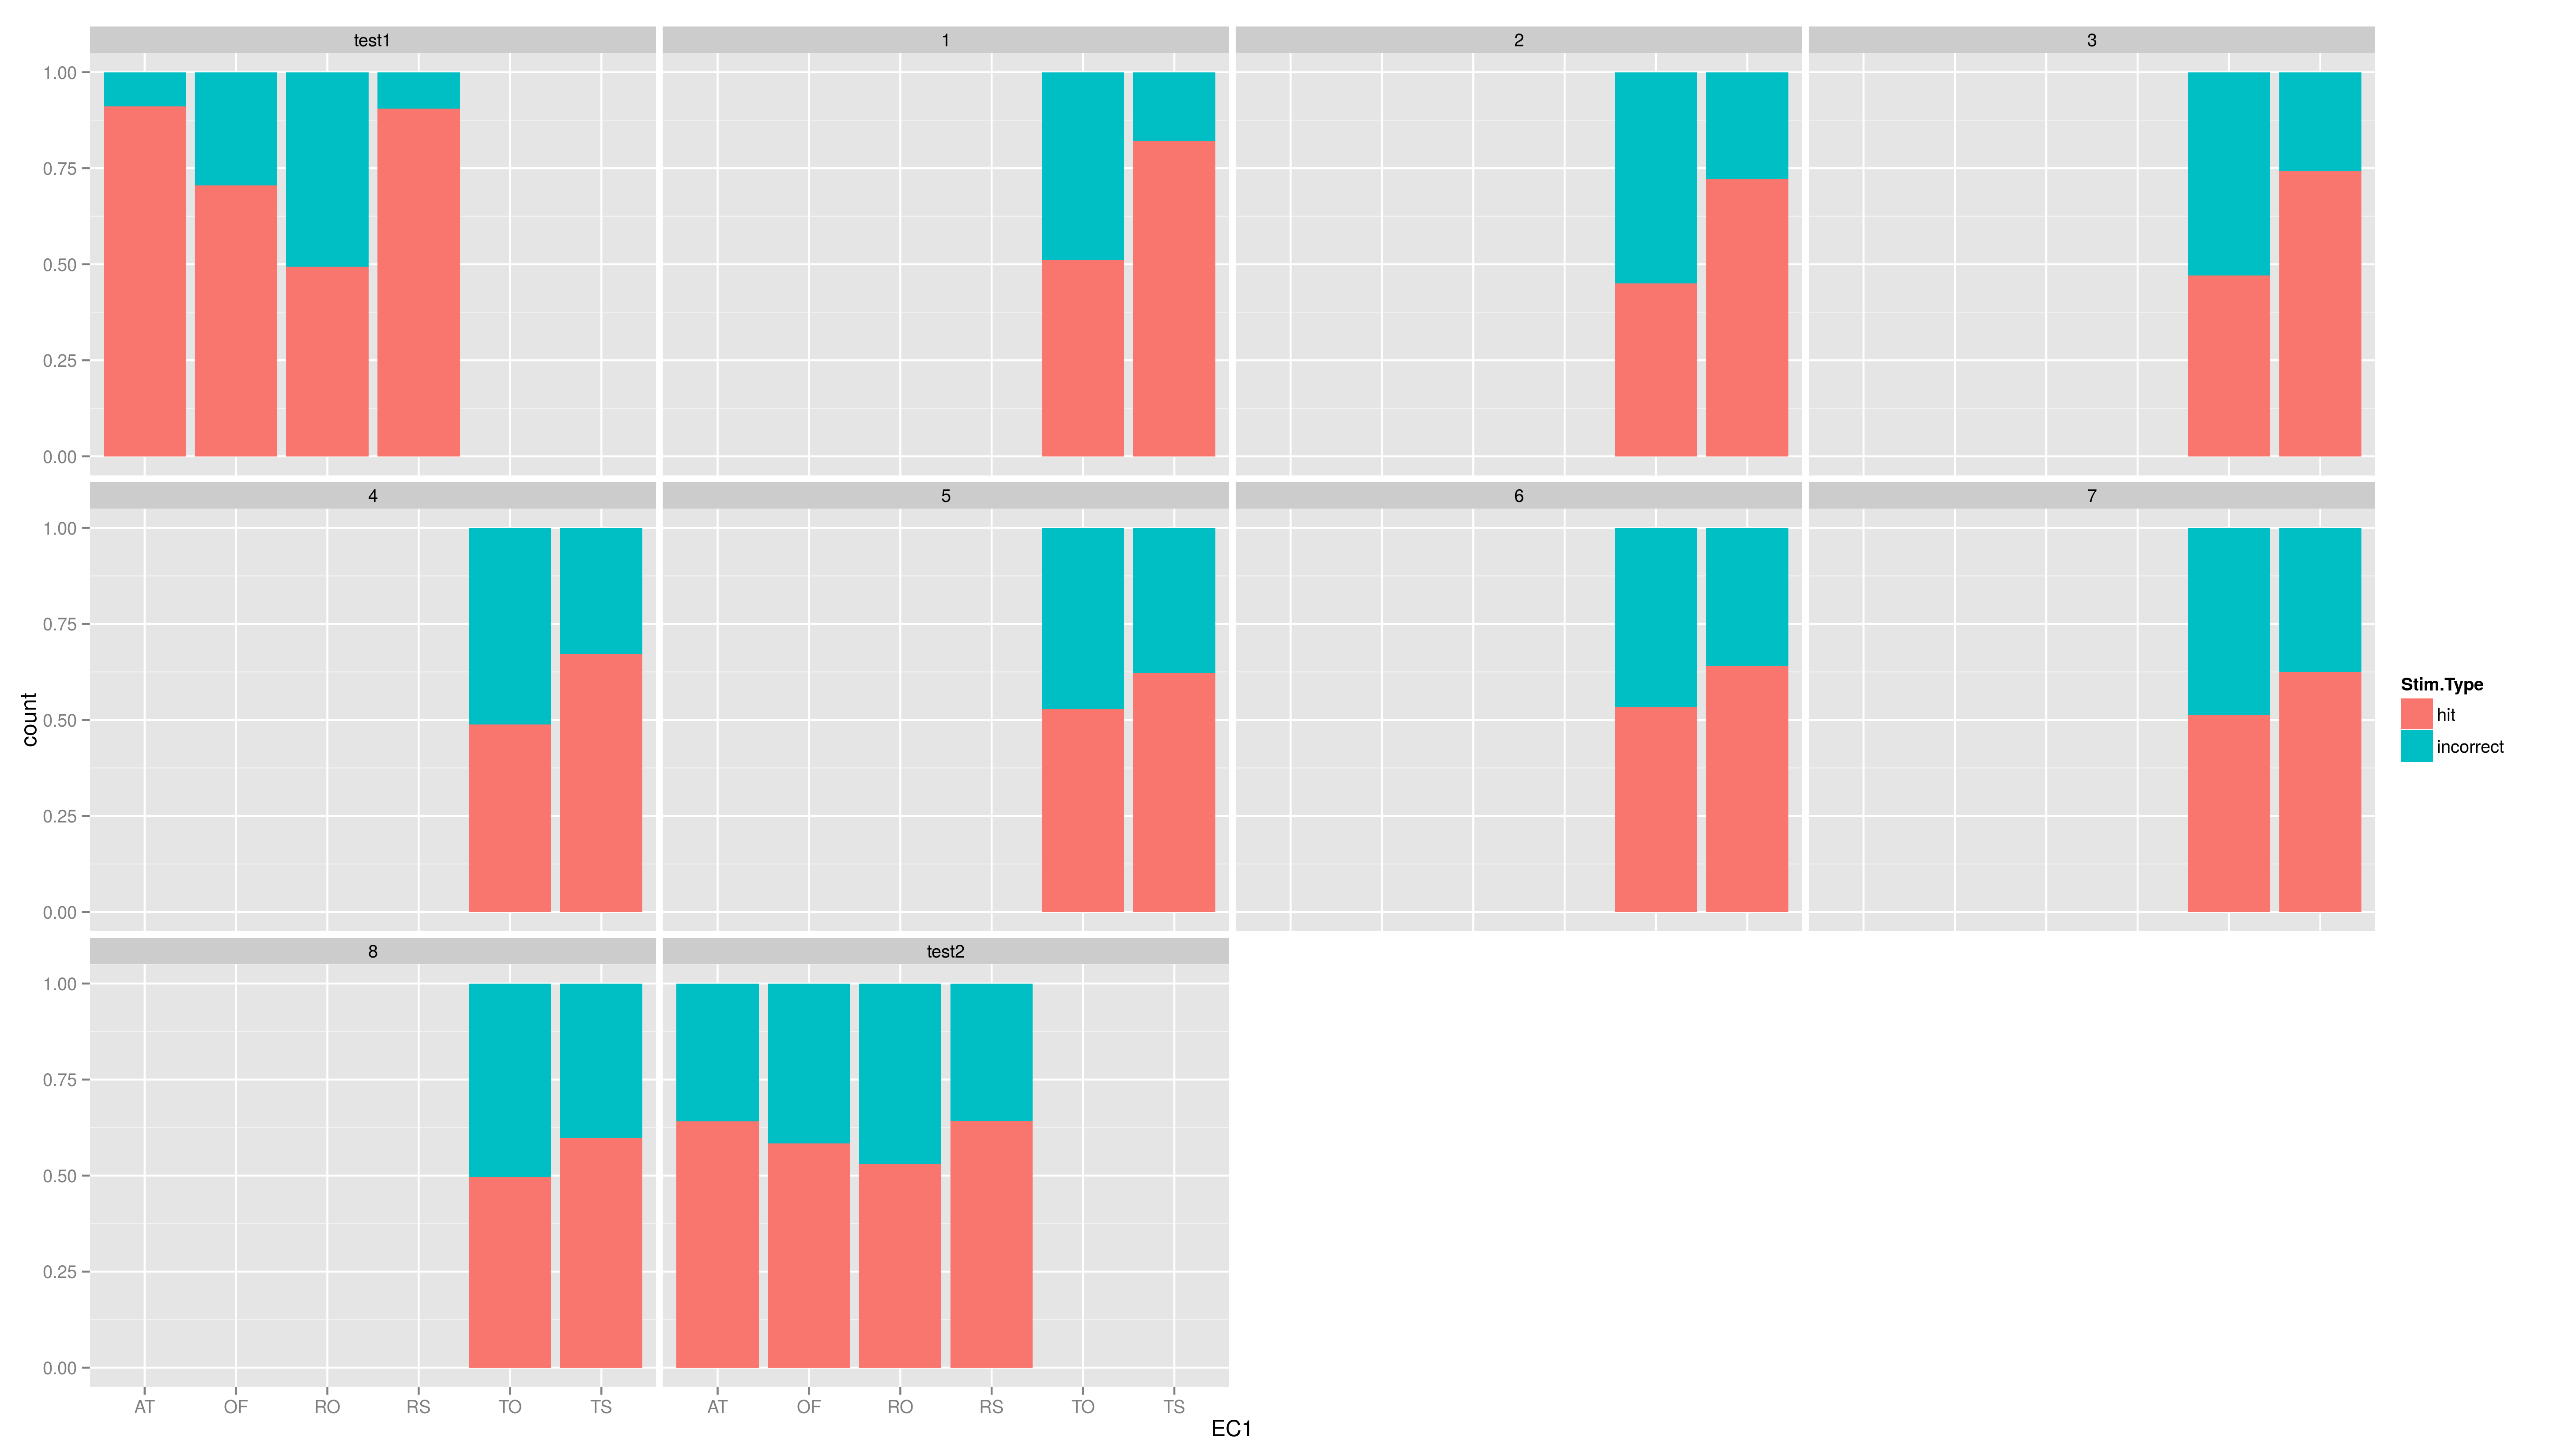
\includegraphics[width=3cm,height=3cm]{plot4.png}}{plot4.png}
\end{center}
\end{frame}


\begin{frame}[fragile]\frametitle{Exercises}
  \begin{itemize}
  \item now add \texttt{facet\_wrap(~testid)} to show the same graph per time
  \end{itemize}
\begin{verbatim}
> ggplot(data,aes(x=EC1,fill=Stim.Type)) +
+     geom_bar(position = "fill") +
+     facet_wrap(~testid,scales = "free")
> 
> ggsave("plot4a.png")
Saving 16 x 9.13 in image
\end{verbatim}
\begin{center}
\linkimage{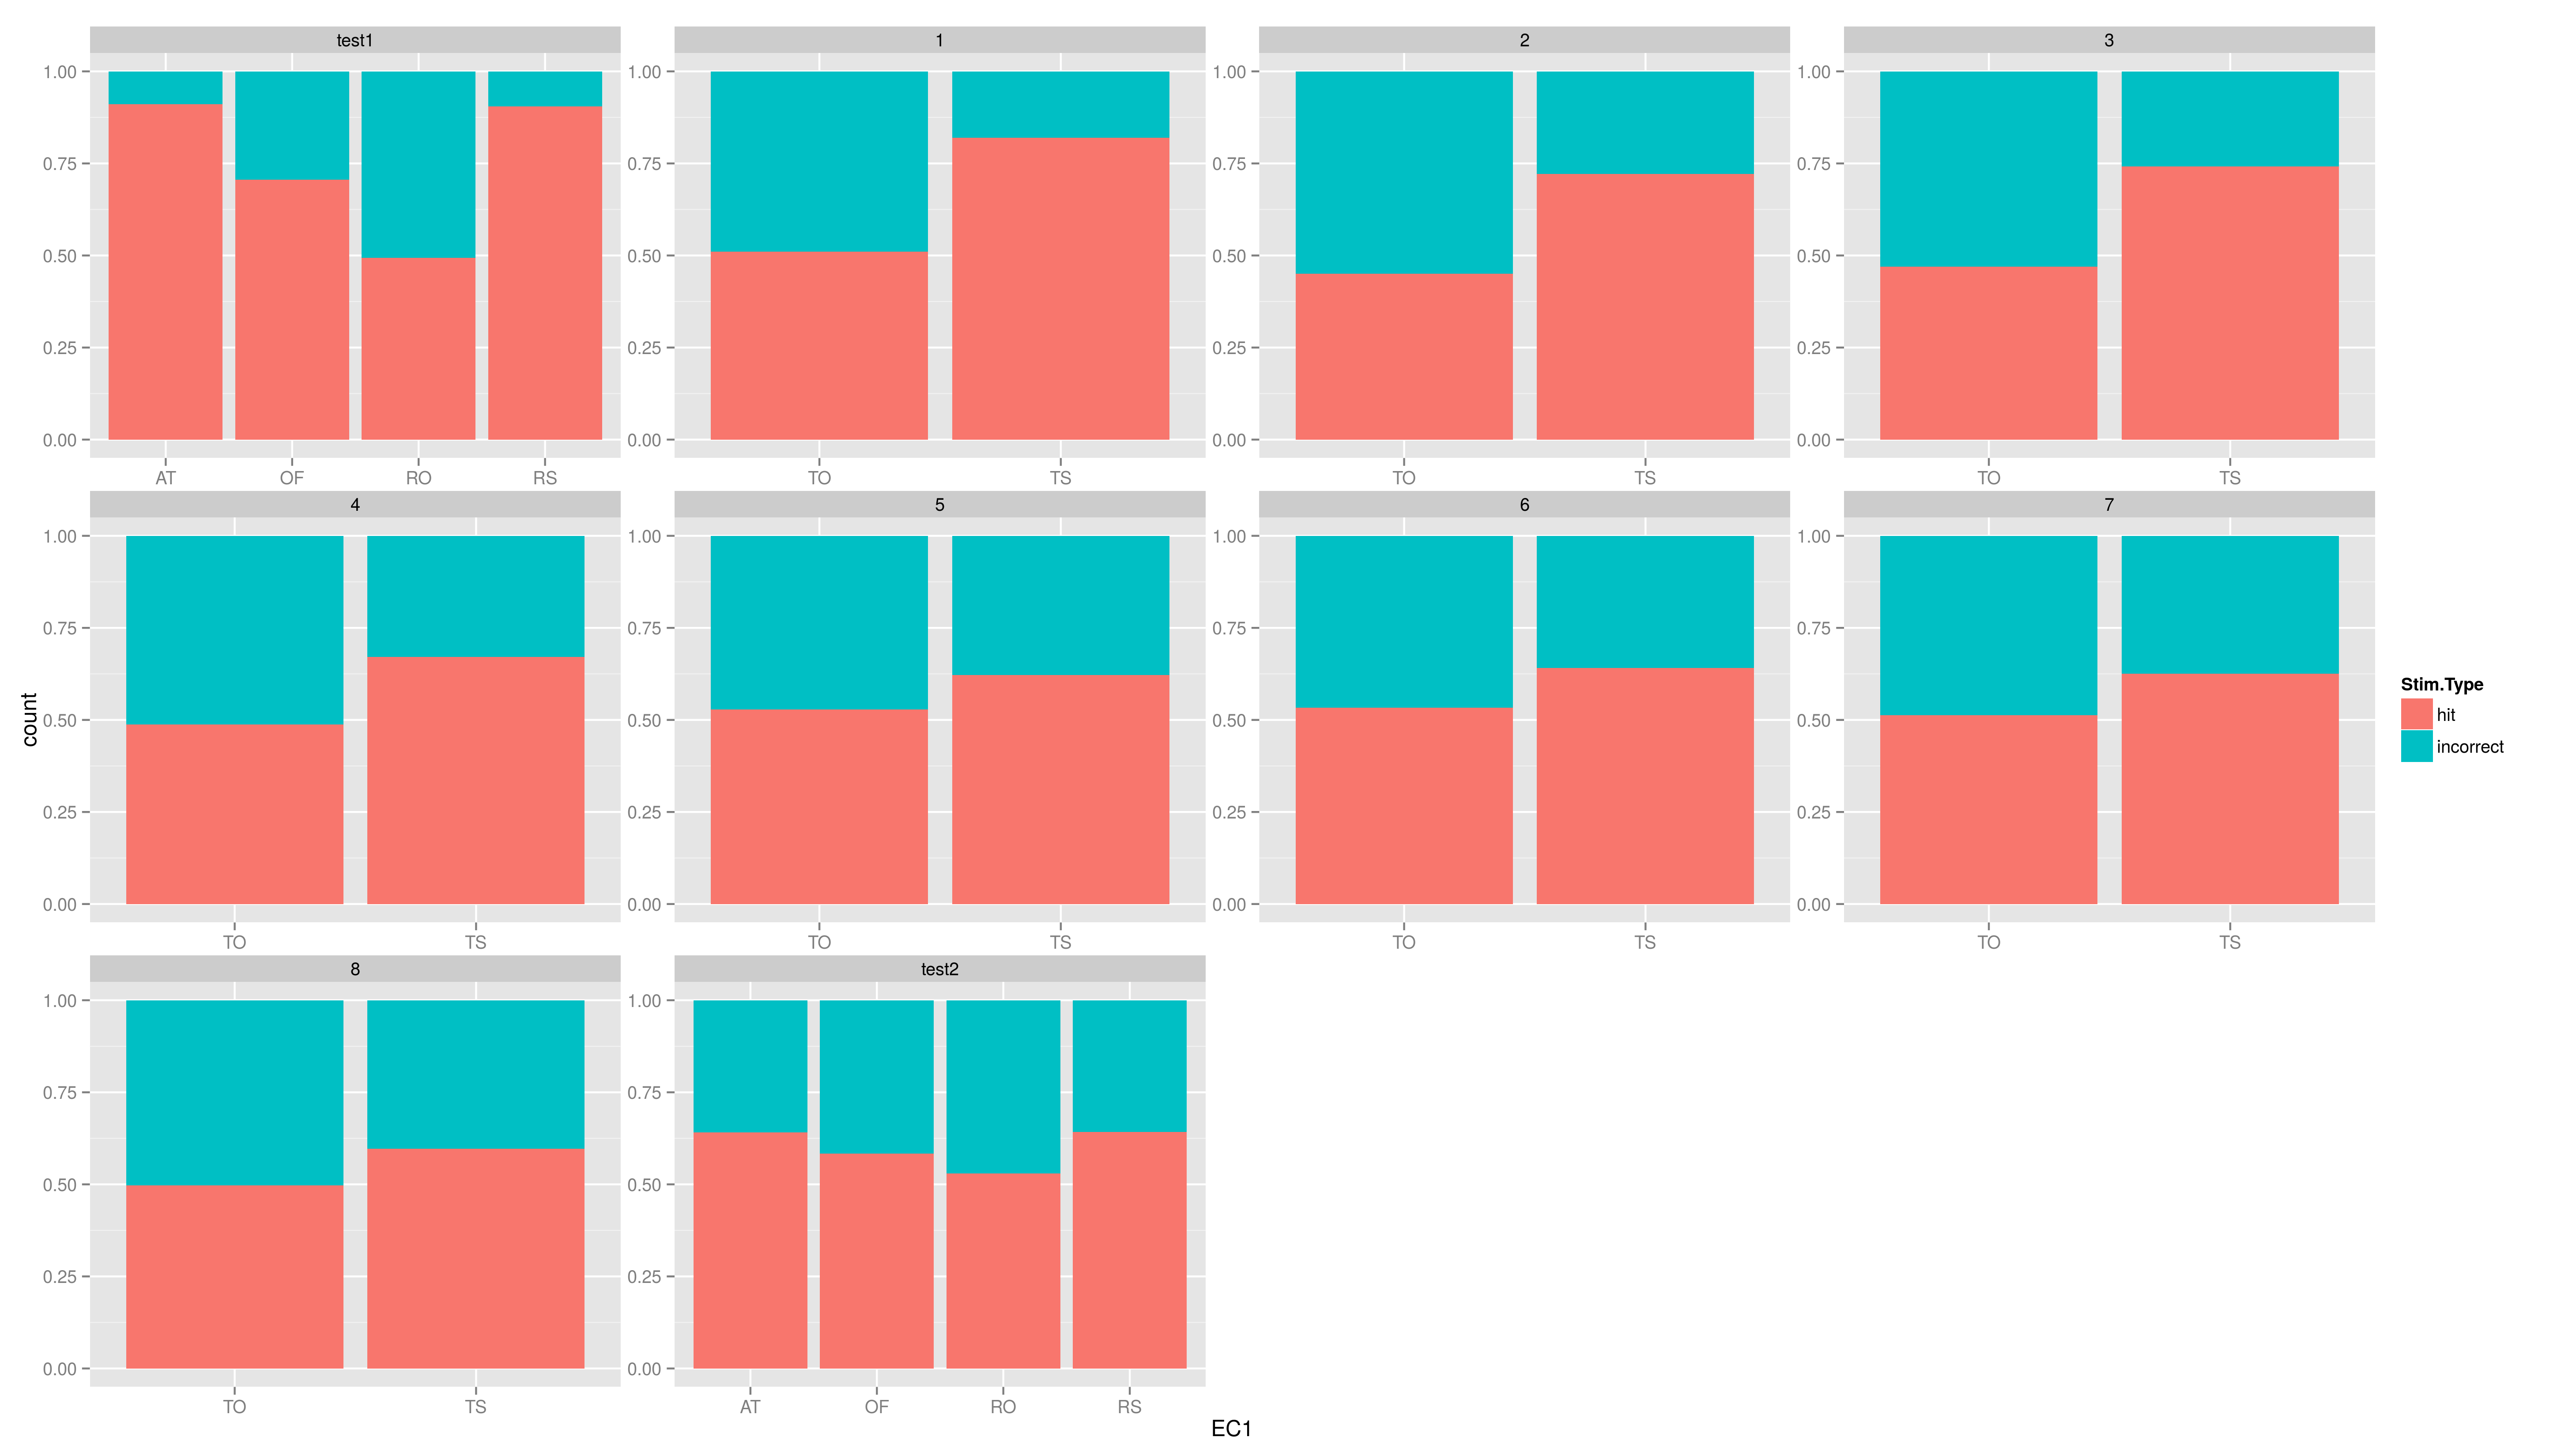
\includegraphics[width=3cm,height=3cm]{plot4a.png}}{plot4a.png}
\end{center}
\end{frame}


\begin{frame}[fragile]\frametitle{Exercises}
  \begin{itemize}
  \item make a graph facetted per child showing stacked hit/incorrect bars with time on the x axis
  \end{itemize}
\begin{verbatim}
> ggplot(data,aes(x=testid,fill=Stim.Type)) +
+     geom_bar(position = "fill") +
+     facet_wrap(~ Subject)
> ggsave("plot5.png")
Saving 16 x 9.13 in image
\end{verbatim}
\begin{center}
\linkimage{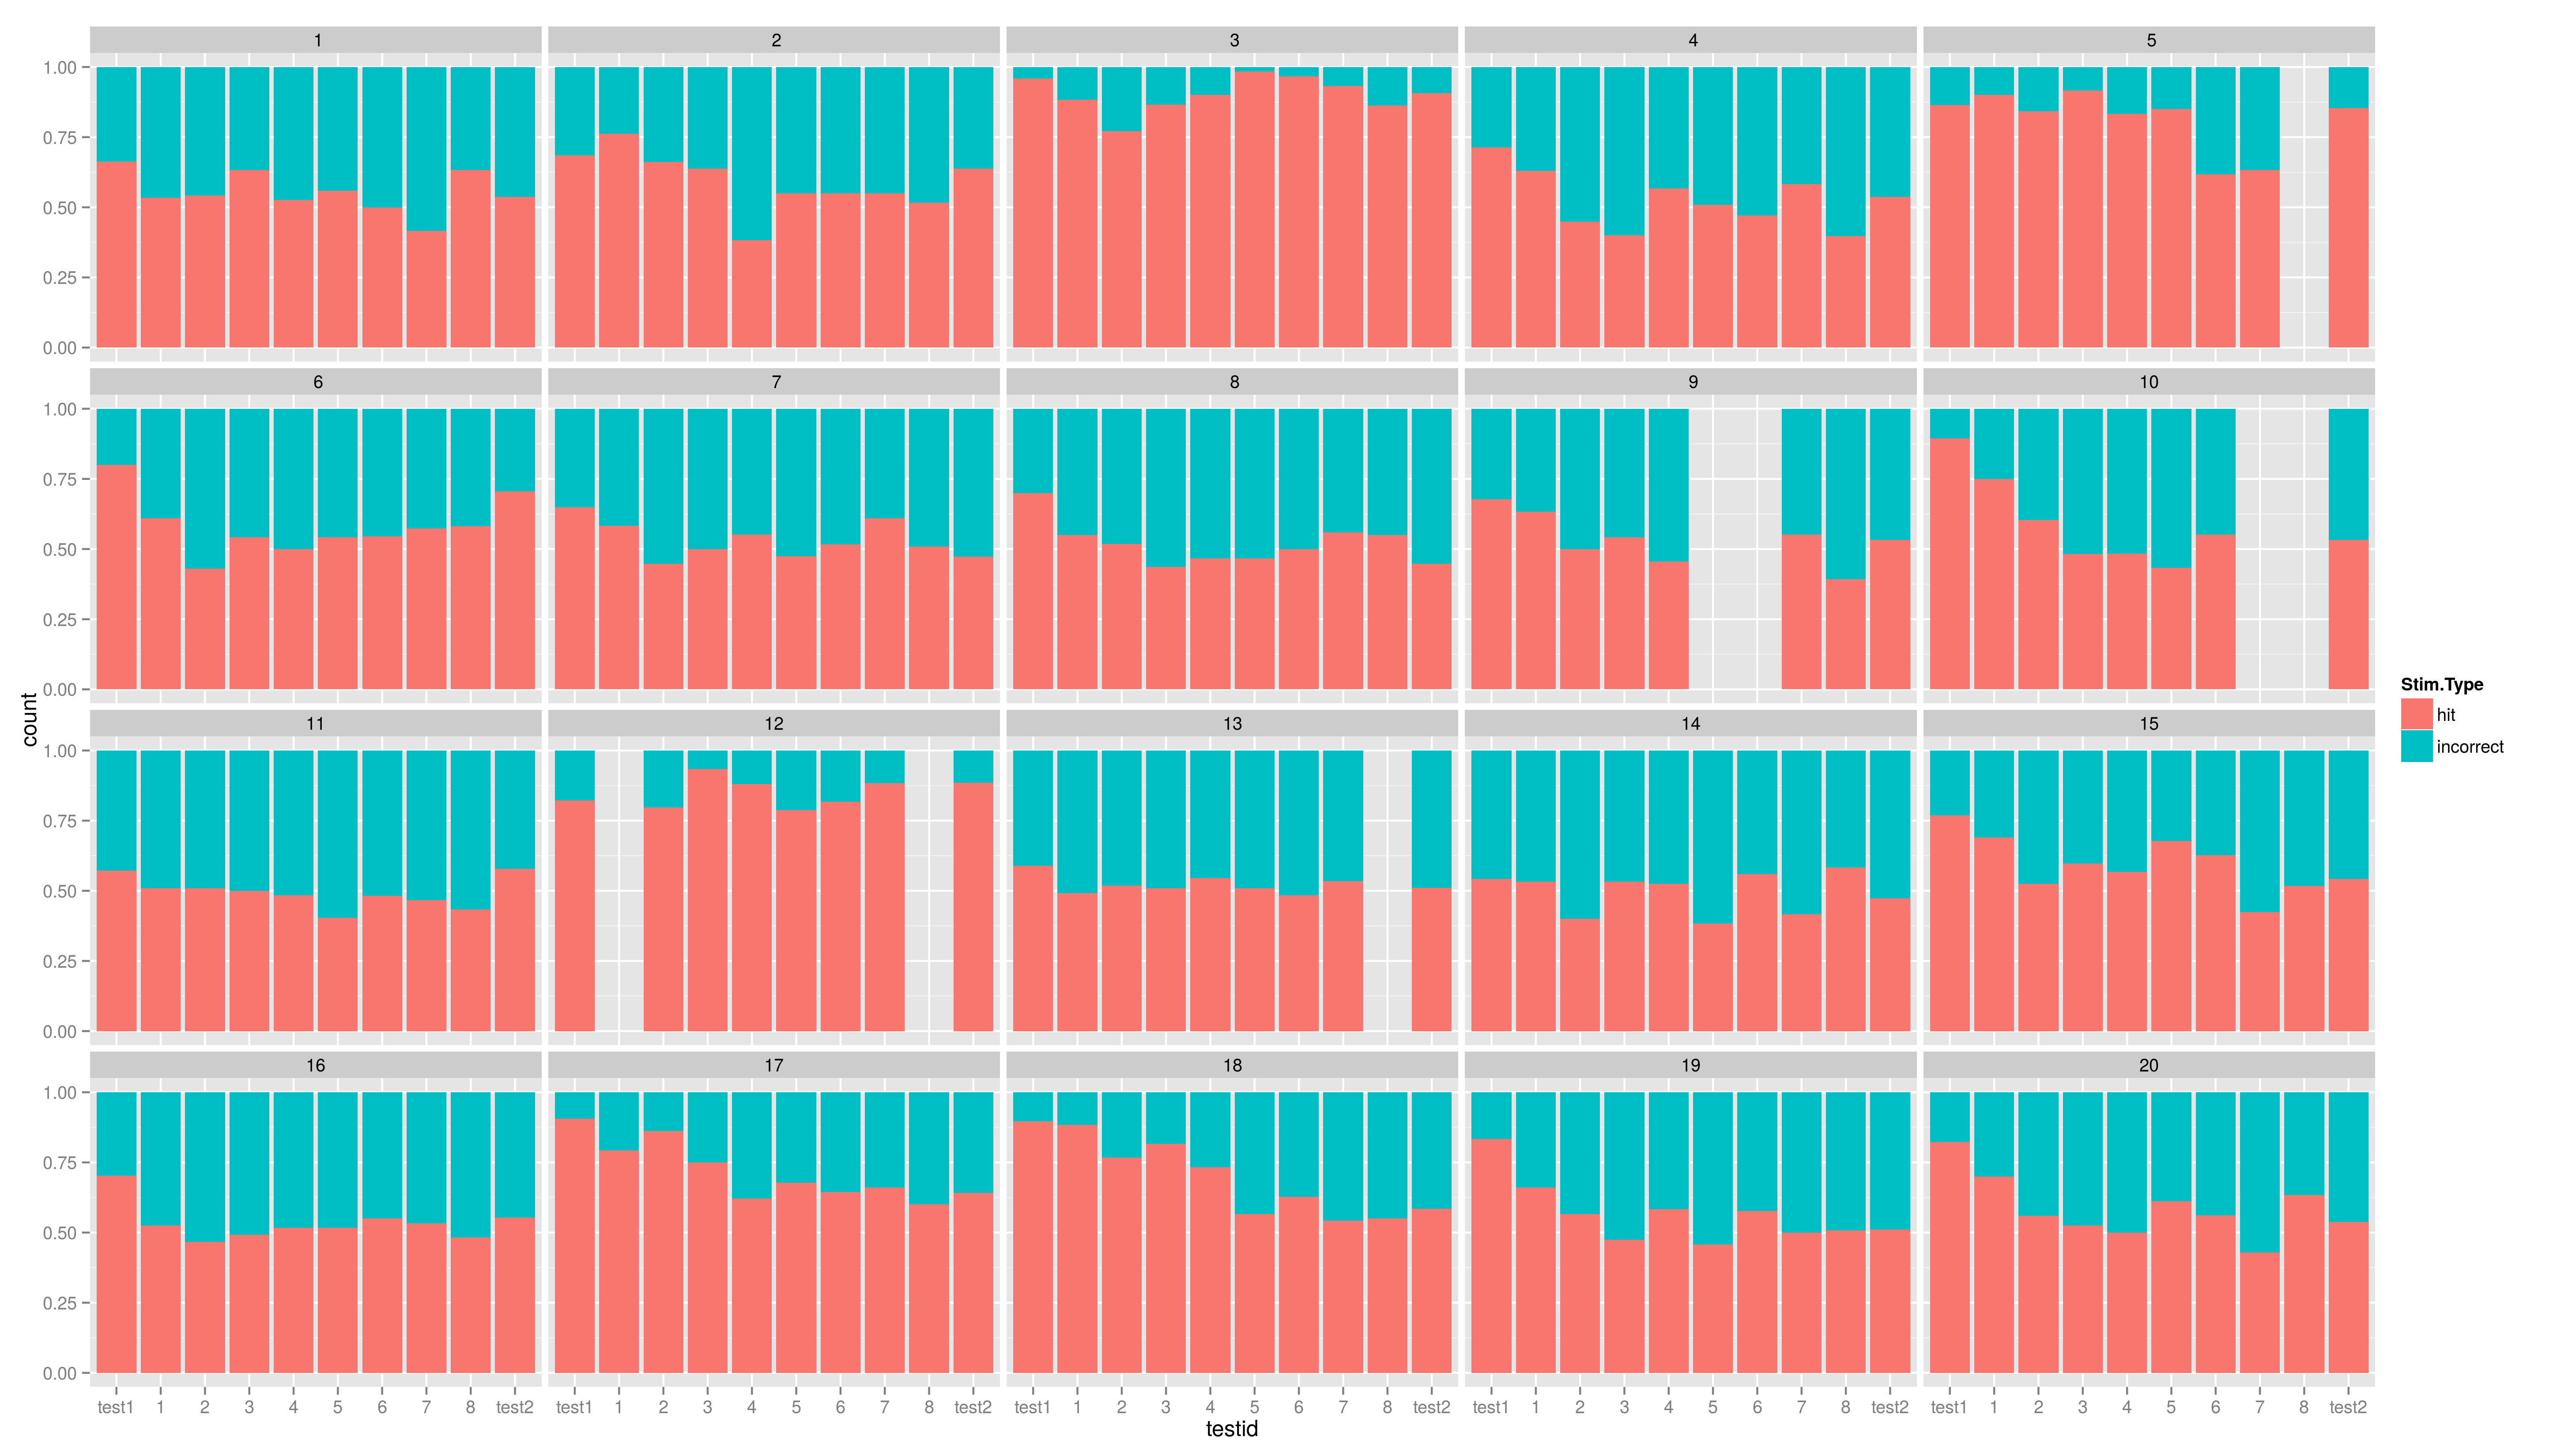
\includegraphics[width=3cm,height=3cm]{plot5.png}}{plot5.png}
\end{center}
\end{frame}


\begin{frame}[fragile]\frametitle{Exercises}
  \begin{itemize}
  \item make a graph facetted per child showing stacked hit/incorrect bars with time on the x axis
  \end{itemize}
\begin{verbatim}
> ggplot(data,aes(x=testid,fill=Stim.Type, y=TTime)) +
+     geom_boxplot() +
+     facet_wrap(~ Subject)
> ggsave("plotbp.png")
Saving 19.3 x 11 in image
\end{verbatim}
\begin{center}
\linkimage{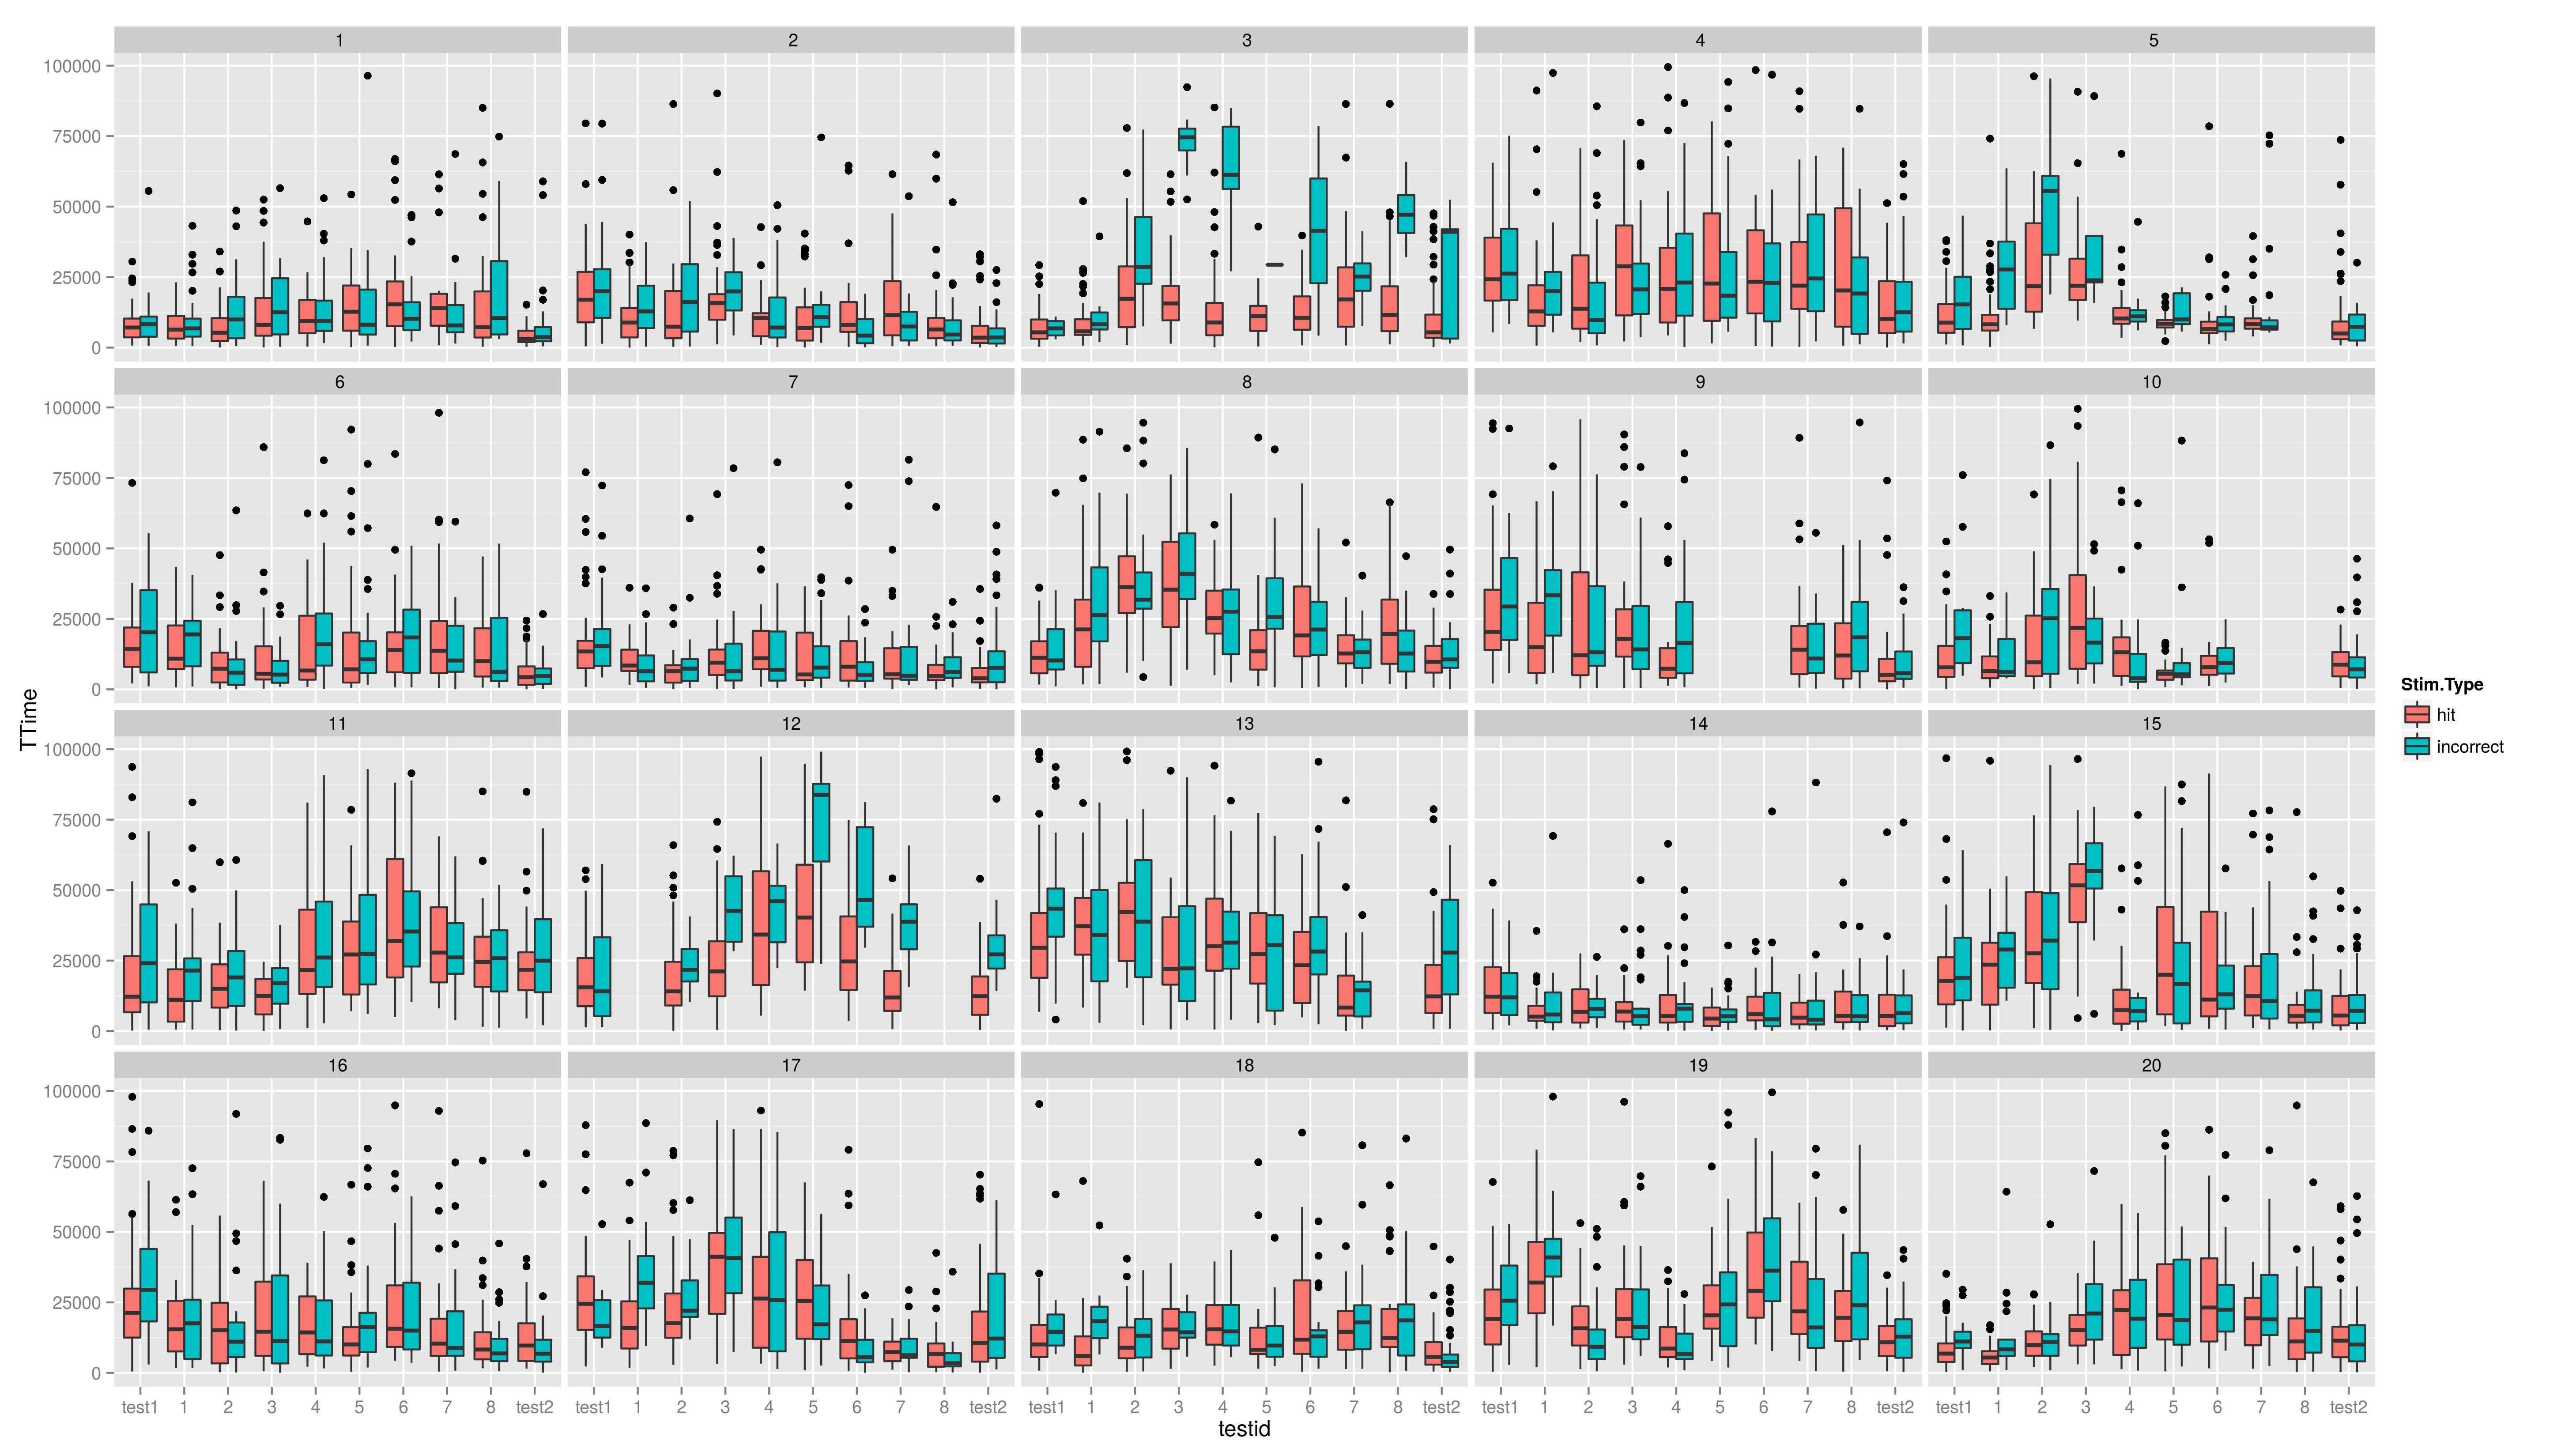
\includegraphics[width=3cm,height=3cm]{plotbp.png}}{plotbp.png}
\end{center}
\end{frame}

\section{dplyr}
\begin{frame}\frametitle{\texttt{Introduction}}
The dplyr package makes each of these steps as fast and easy as possible by:
\begin{itemize}
\item  Elucidating the most common data manipulation operations, so that your options are helpfully constrained when thinking about how to tackle a problem.
\item  Providing simple functions that correspond to the most common data manipulation verbs, so that you can easily translate your thoughts into code.
\item Using efficient data storage backends, so that you spend as little time waiting for the computer as possible.
\end{itemize}
\end{frame}

\subsection{filter()}
\begin{frame}[fragile]\frametitle{\texttt{filter()}}
  \begin{itemize}
  \item  Base R approach to filtering forces you to repeat the data frame’s name
  \item dplyr approach is simpler to write and read
  \item Command structure (for all dplyr verbs):
    \begin{itemize}
    \item first argument is a data frame
    \item return value is a data frame
    \item nothing is modified in place
    \end{itemize}
  \item Note: dplyr generally does not preserve row names
  \end{itemize}
\end{frame}


\begin{frame}[fragile]\frametitle{\texttt{filter() example}}\footnotesize
\begin{verbatim}
> require(dplyr)
> sub1 <- filter(data, Subject == 1)
> table(sub1$Subject)

  1 
665   
> sub1 <- filter(data, Subject == 1, Stim.Type == "incorrect")
> table(sub1$Subject,sub1$Stim.Type)
   
    hit incorrect other miss
  1   0       293     0    0
> subframe <- filter(data, Age_PRETEST < 3.5 | Sex == "m" )
> table(subframe$Age_PRETEST < 3.5, subframe$Sex)
       
           f    m
  FALSE    0 3202
  TRUE  1333 1844
\end{verbatim}
\end{frame}


\subsection{select()}
\begin{frame}[fragile]\frametitle{\texttt{select()}}
  \begin{itemize}
  \item \texttt{select()} selects colums
  \item it can be used in combination with \texttt{filter()}
  \item combining can be done by the infix $\%>\%$
  \end{itemize}
\end{frame}

\begin{frame}[fragile]\frametitle{\texttt{select() example}}\footnotesize
\begin{verbatim}
> subframe <- select(data, Subject, Sex, Age_PRETEST)
> head(subframe)
  Subject Sex Age_PRETEST
1       1   f        3.11
2       1   f        3.11
3       1   f        3.11
4       1   f        3.11
5       1   f        3.11
6       1   f        3.11
> subframe <- select(data, Subject, Sex, Age_PRETEST) %>%
+     filter(Age_PRETEST < 3.2)
> table(subframe$Subject)

  1   4   9  16  18 
665 645 536 663 668 
\end{verbatim}
\end{frame}

\subsection{arrange()}
\begin{frame}[fragile]\frametitle{\texttt{arrange()}}
  \begin{itemize}
  \item arrange can be used to change the order of rows
  \end{itemize}\tiny
\begin{verbatim}
> arr.frame <- arrange(data, TTime, Time)
> head(arr.frame)
  Subject Sex Age_PRETEST Trial Event.Type Code     Time TTime Uncertainty
1       2   m        4.50   255   Response    1  9250486     2           1
2      15   f        4.11   381   Response    2  7850406    10           1
3      14   m        4.60   297   Response    1 11254989    13           1
4      17   m        4.90   234   Response    2 12267915    13           1
5       9   m        3.11   127   Response    1  1445239    16           1
6       2   m        4.50   332   Response    2  3580014    24           1
  Duration Uncertainty.1 ReqTime ReqDur Stim.Type Pair.Index    Type Event.Code
1      200             2       0   next       hit        220 Picture   TO18.jpg
2      200             2       0   next       hit        328 Picture   TO22.jpg
3      200             2       0   next       hit        258 Picture   TS05.jpg
4      200             2       0   next incorrect        202 Picture   TO03.jpg
5      200             2       0   next       hit        126 Picture   RS21.jpg
6      200             2       0   next       hit        333 Picture   RS30.jpg
     Time1 testid EC1
1  9250484      1  TO
2  7850396      4  TO
3 11254976      5  TS
4 12267902      6  TO
5  1445223  test2  RS
6  3579990  test2  RS  
\end{verbatim}
\end{frame}


\subsection{mutate() and transmute()}
\begin{frame}[fragile]\frametitle{\texttt{mutate()}}
  \begin{itemize}
  \item \texttt{mutate()} can be used to transform or add columns
  \item you can add/change more than one column at once
  \end{itemize}
\end{frame}


\begin{frame}[fragile]\frametitle{\texttt{mutate() example}}\tiny
\begin{verbatim}
> subframe <- filter(data, Subject == 1) %>%
+     mutate(Event.Code = str_replace(Event.Code,".jpg",""),
+            TTime.calc = Time - Time1)
> head(subframe)
  Subject Sex Age_PRETEST Trial Event.Type Code   Time TTime Uncertainty
1       1   f        3.11     7   Response    2 103745  2575           1
2       1   f        3.11    12   Response    2 156493  2737           1
3       1   f        3.11    17   Response    2 214772  6630           1
4       1   f        3.11    22   Response    1 262086  5957           1
5       1   f        3.11    27   Response    2 302589   272           1
6       1   f        3.11    32   Response    1 352703  7197           1
  Duration Uncertainty.1 ReqTime ReqDur Stim.Type Pair.Index    Type Event.Code
1     2599             3       0   next       hit          7 Picture       RO26
2     2800             2       0   next incorrect         12 Picture       RO19
3     6798             2       0   next       hit         17 Picture       RS23
4     5999             2       0   next incorrect         22 Picture       OF22
5      400             2       0   next       hit         27 Picture       AT08
6     7398             2       0   next       hit         32 Picture       AT30
   Time1 testid EC1 TTime.calc
1 101170  test2  RO       2575
2 153756  test2  RO       2737
3 208142  test2  RS       6630
4 256129  test2  OF       5957
5 302317  test2  AT        272
6 345506  test2  AT       7197
> table(subframe$Subject)

  1 
665   
\end{verbatim}
\end{frame}

\begin{frame}[fragile]\frametitle{\texttt{transmute()}}
  \begin{itemize}
  \item \texttt{transmute()} does the same like \texttt{mutate{}} but keeps only the new columns
  \end{itemize}\footnotesize
\begin{verbatim}
> mut.frame <- transmute(data,
+                     Event.Code = str_replace(Event.Code,".jpg",""),
+                     TTime.calc = Time - Time1)
> head(mut.frame)
  Event.Code TTime.calc
1       RO26       2575
2       RO19       2737
3       RS23       6630
4       OF22       5957
5       AT08        272
6       AT30       7197
\end{verbatim}
\end{frame}

\subsection{summarise()}
\begin{frame}[fragile]\frametitle{\texttt{summarise()}}
  \begin{itemize}
  \item \texttt{summarise()} makes summary statistics
  \end{itemize}
\begin{verbatim}
> sum.frame <- summarise(data, mean.ttime=mean(TTime), sd.ttime = sd(TTime))
> sum.frame
  mean.ttime sd.ttime
1   18393.74 17876.12  
\end{verbatim}
\end{frame}


\begin{frame}[fragile]\frametitle{\texttt{summarise()} example}
  \begin{itemize}
  \item \texttt{summarise()} gets really interesting in combination with \texttt{group\_by()} also included in the \texttt{dplyr} package
  \end{itemize}\footnotesize
\begin{verbatim}
> sum.frame <- group_by(data, Subject) %>%
+     summarise(mean.ttime=mean(TTime), sd.ttime = sd(TTime))
> sum.frame
Source: local data frame [20 x 3]

   Subject mean.ttime sd.ttime
1        1  11717.854 13035.85
2        2  13100.568 13607.71
3        3  15709.598 16464.09
4        4  24778.592 20205.91
5        5  14759.785 14863.84
6        6  14081.377 14834.64
7        7  11551.482 12814.57
8        8  22739.310 18215.68
9        9  20490.722 19399.49
...
\end{verbatim}
\end{frame}


\begin{frame}[fragile]\frametitle{\texttt{summarise()} example}
\footnotesize
\begin{verbatim}
> sum.frame <- group_by(data, Subject, testid) %>%
+     summarise(mean.ttime=mean(TTime), sd.ttime = sd(TTime))
> head(sum.frame)
Source: local data frame [6 x 4]
Groups: Subject

  Subject testid mean.ttime  sd.ttime
1       1  test1   8621.674  7571.462
2       1      1   9256.367  8682.833
3       1      2   9704.712 10479.788
4       1      3  14189.550 13707.021
5       1      4  13049.831 11344.656
6       1      5  14673.525 15575.355
...
\end{verbatim}
\end{frame}


\section{ggplot2 - Part 2}
\subsection{scales and themes}

\begin{frame}[fragile]\frametitle{Scales}
What if we want to change the colours?
\begin{itemize}
\item this leads to another important type of component not yet mentioned
\item if you map a variable to a aesthetic is these done in a default way, in this case some reddish colour is mapped to \texttt{hit} while light blue is mapped to \texttt{incorrect}; in addition a discrete range of colours is automatically used
\item these rules of mapping are called \texttt{scales}
\item different type of scales exists for the axes, colours, shapes etc, some of them exists in discrete and continuous versions, some in just one of them (in general one can say, everytime there can be a legend there is a scale)
\item the name convention: scale\_aesthetic\_specification. for example scale\_x\_discrete for customizing a discrete x axis (e.g. in barplots)
\end{itemize}
\end{frame}


\begin{frame}[fragile]\frametitle{Changing a Scale}
  \begin{itemize}
  \item to change our discrete colour scale for the filling we type \footnotesize
\begin{verbatim}
> ggplot(data,aes(x=EC1,fill=Stim.Type)) +
+     geom_bar(position = "fill") +
+     facet_wrap(~testid,scales = "free") +
+     scale_fill_manual(values=c("forestgreen","firebrick"))
\end{verbatim}
  \end{itemize}
\begin{center}
\linkimage{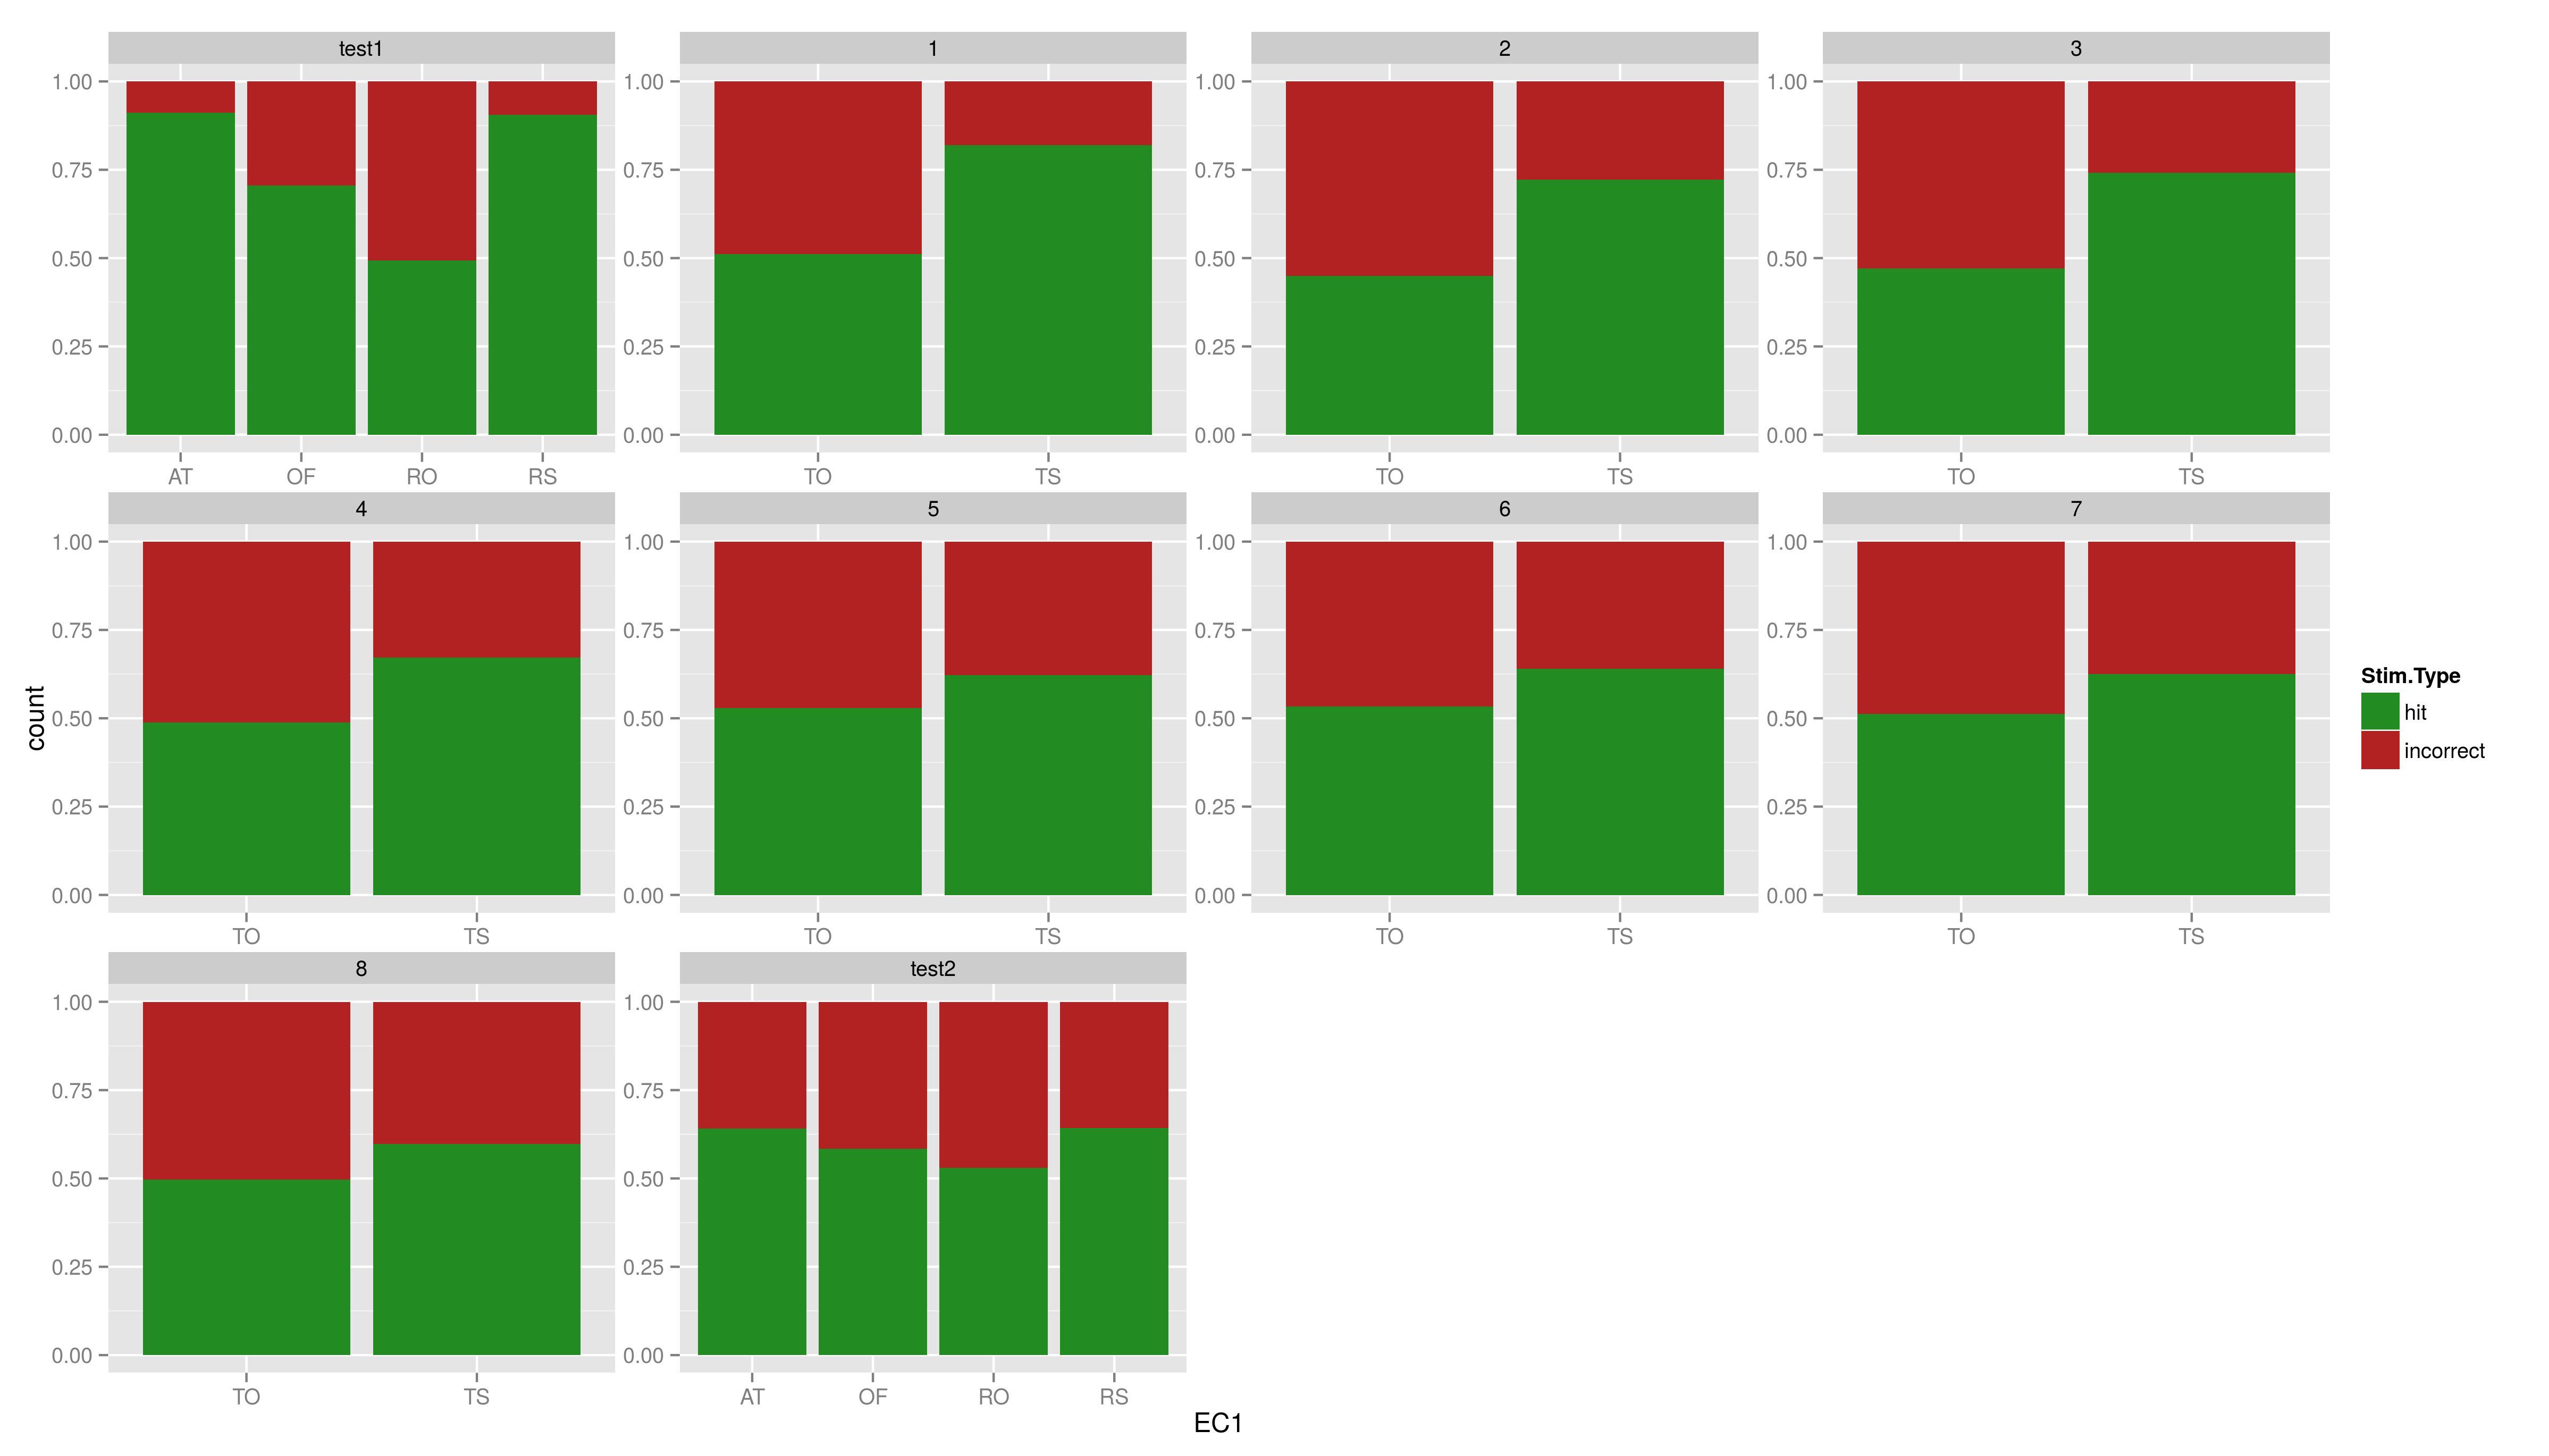
\includegraphics[width=5cm,height=5cm]{ggp10.png}}{ggp10.png}
\end{center}
\end{frame}


\begin{frame}[fragile]\frametitle{Changing a Scale}
There are other ways to customize a discrete colour/fill scales
  \begin{itemize}
  \item \texttt{scale\_colour\_grey()}
  \item \texttt{scale\_colour\_hue()}
  \item \texttt{scale\_colour\_brewer()}
  \end{itemize}
\end{frame}

\begin{frame}[fragile]\frametitle{Changing a Scale}
\begin{verbatim}
> ggplot(data,aes(x=EC1,fill=Stim.Type)) +
+     geom_bar(position = "fill") +
+     facet_wrap(~testid,scales = "free") +
+         scale_fill_grey()
> ggplot(data,aes(x=EC1,fill=Stim.Type)) +
+     geom_bar(position = "fill") +
+     facet_wrap(~testid,scales = "free") +
+         scale_fill_hue(h=c(180,360))
> ggplot(data,aes(x=EC1,fill=Stim.Type)) +
+     geom_bar(position = "fill") +
+     facet_wrap(~testid,scales = "free") +
+     scale_fill_brewer(type = "div",palette = 2)
\end{verbatim}
\end{frame}


\section{stringr}
%% \subsection{Characteristics}
%% \begin{frame}\frametitle{\texttt{str\_lenght()}}

%% \end{frame}


%% \subsection{Extract/Replace Substrings}
%% \begin{frame}\frametitle{\texttt{str\_extract()}}

%% \end{frame}

%% \begin{frame}\frametitle{\texttt{str\_sub()}}

%% \end{frame}

%% \begin{frame}\frametitle{\texttt{str\_detect()}}

%% \end{frame}

%% \begin{frame}\frametitle{\texttt{str\_locate()}}

%% \end{frame}

%% \begin{frame}\frametitle{\texttt{str\_trim()}}

%% \end{frame}

%% \begin{frame}\frametitle{\texttt{str\_replace()}}

%% \end{frame}


%% \subsection{Other}
%% \begin{frame}\frametitle{\texttt{str\_dup()}}

%% \end{frame}

%% \begin{frame}\frametitle{\texttt{str\_pad()}}

%% \end{frame}

%% \begin{frame}\frametitle{\texttt{str\_c()}}

%% \end{frame}

%% \begin{frame}\frametitle{\texttt{str\_wrap()}}

%% \end{frame}




\appendix
\flushlinkimages

\end{document}
